\documentclass{article}
\usepackage[spanish]{babel}
\usepackage{graphicx}
\usepackage{xcolor}
\usepackage[utf8]{inputenc}
\usepackage{fancyhdr}
\usepackage{lastpage}
\usepackage{enumitem}
\usepackage{listings}
\usepackage{float}
\usepackage{verbatim}

\pagestyle{fancy}
\fancyhf{}
\rfoot{Page \thepage\hspace{1pt} de~\pageref{LastPage}}

\title{Práctica Tika Apache}
\author{Guillermo López García}
\begin{document}

%\lstset{language=, texcl=true}
%\begin{lstlisting}[frame=single]
%\end{lstlisting}

\textbf{Ejercicios.}
\begin{enumerate}
    \item El autor es `Lo'.
        \begin{figure}[H]
        \centering
        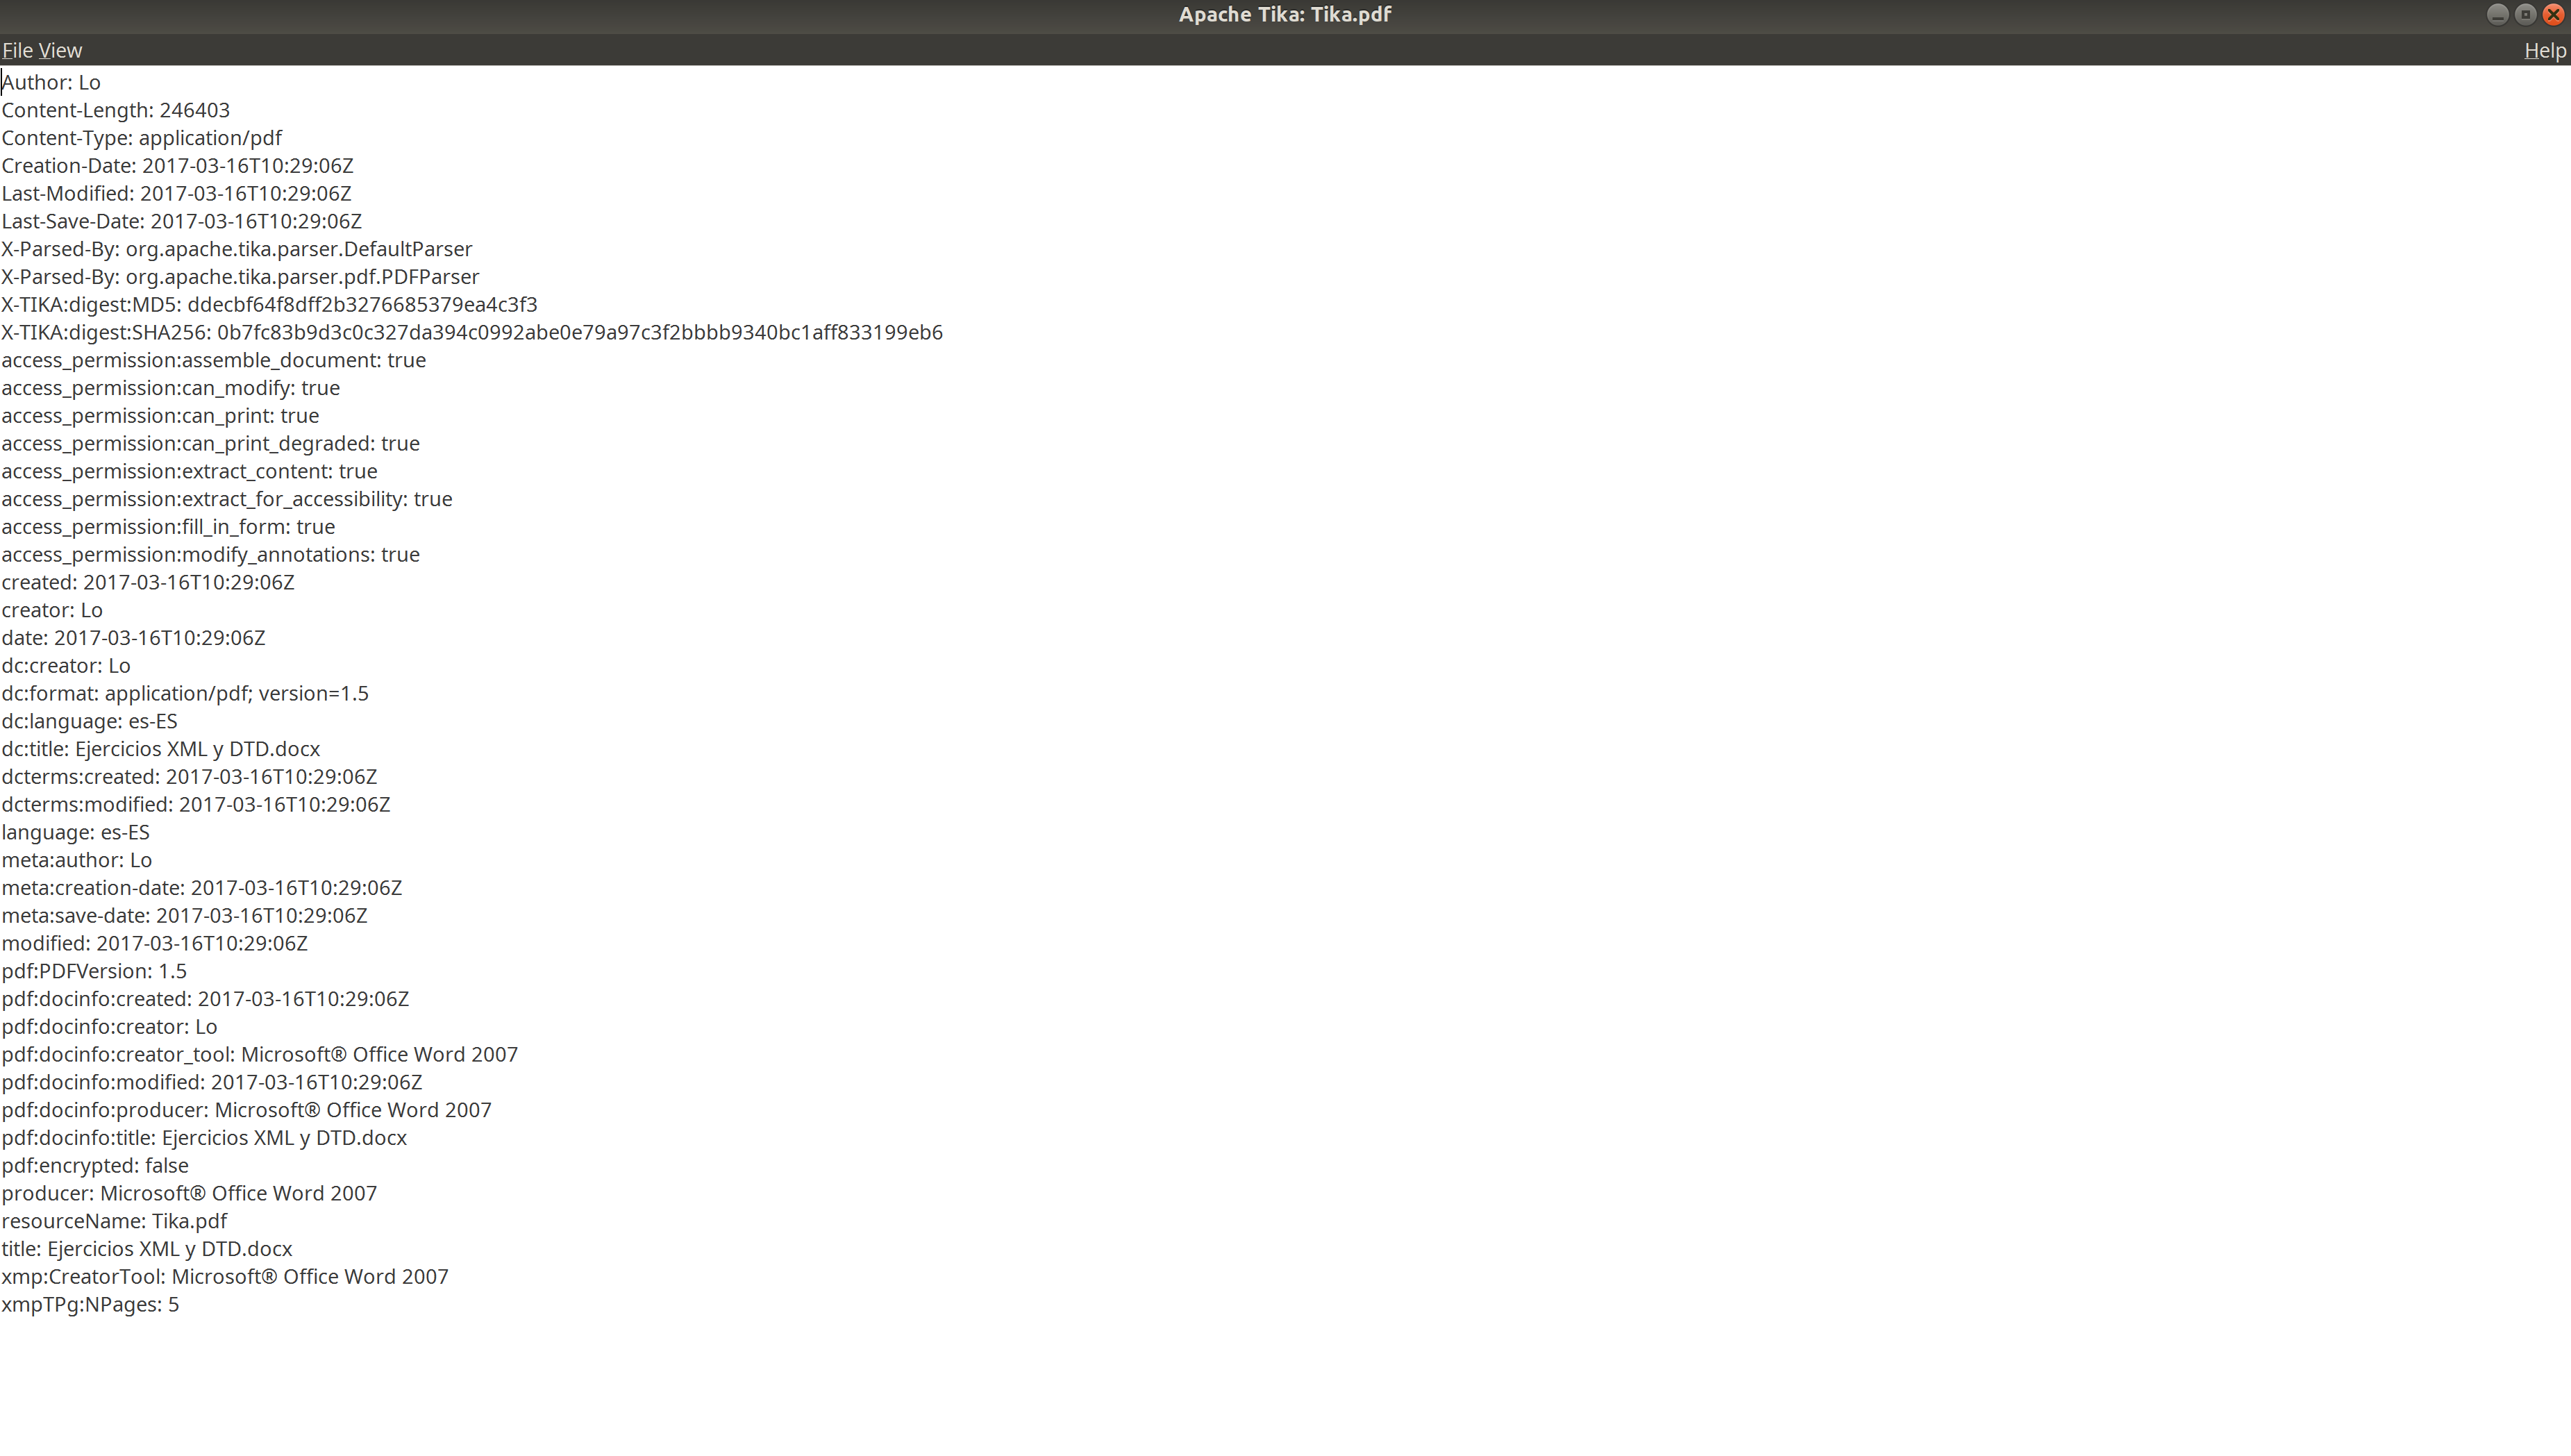
\includegraphics[width=0.7\linewidth]{./ej1}
        \caption{Ejercicio 1.}
        \end{figure}
    \item tika --text-main Tika.pdf $>$ Tika.doc
        \begin{figure}[H]
        \centering
        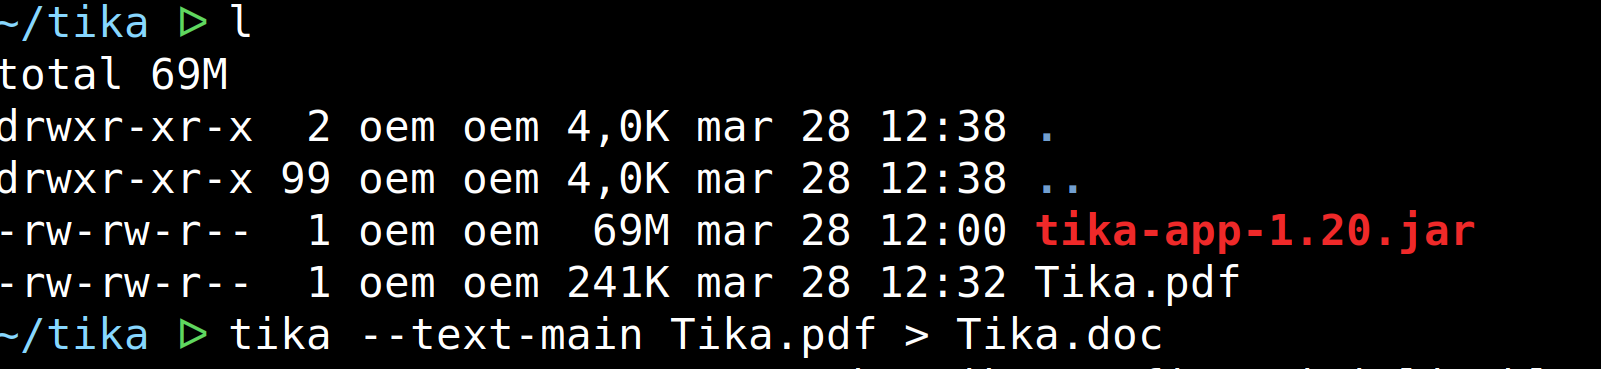
\includegraphics[width=0.7\linewidth]{./ej2}
        \caption{Ejercicio 2.}
        \end{figure}
    \item tika --metadata https://www.uca.es
        \begin{figure}[H]
        \centering
        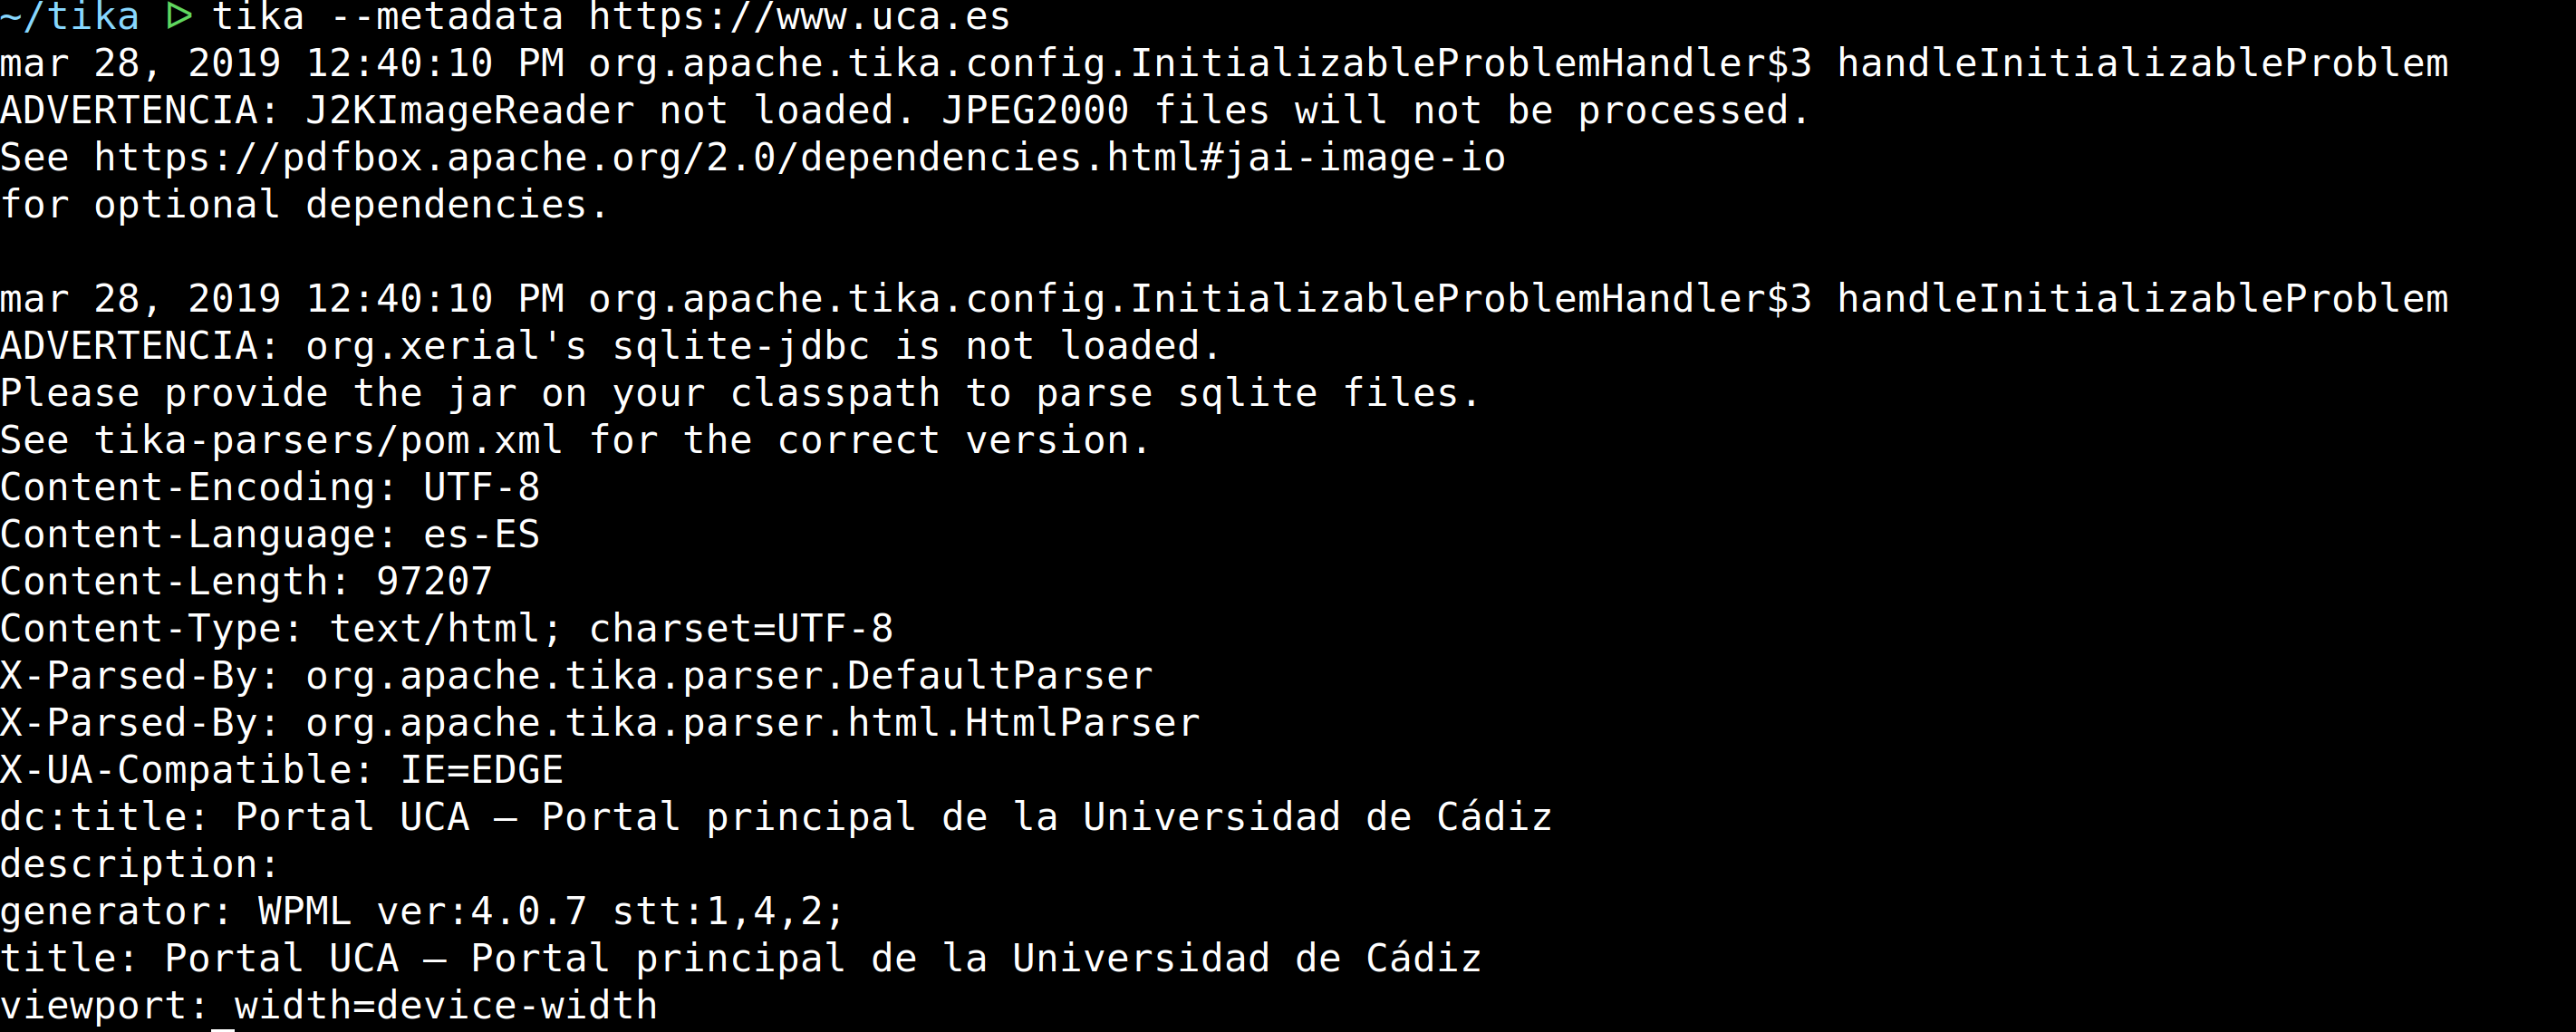
\includegraphics[width=0.7\linewidth]{./ej3}
        \caption{Ejercicio 3.}
        \end{figure}
    \item
        \begin{enumerate}
            \item echo `Archivo de texto plano listo para comprimir.' $>$ archivo.txt
            \item cat archivo.txt
            \item zip archivo.zip archivo.txt
            \item tika --detect archivo.zip
                \begin{figure}[H]
                \centering
                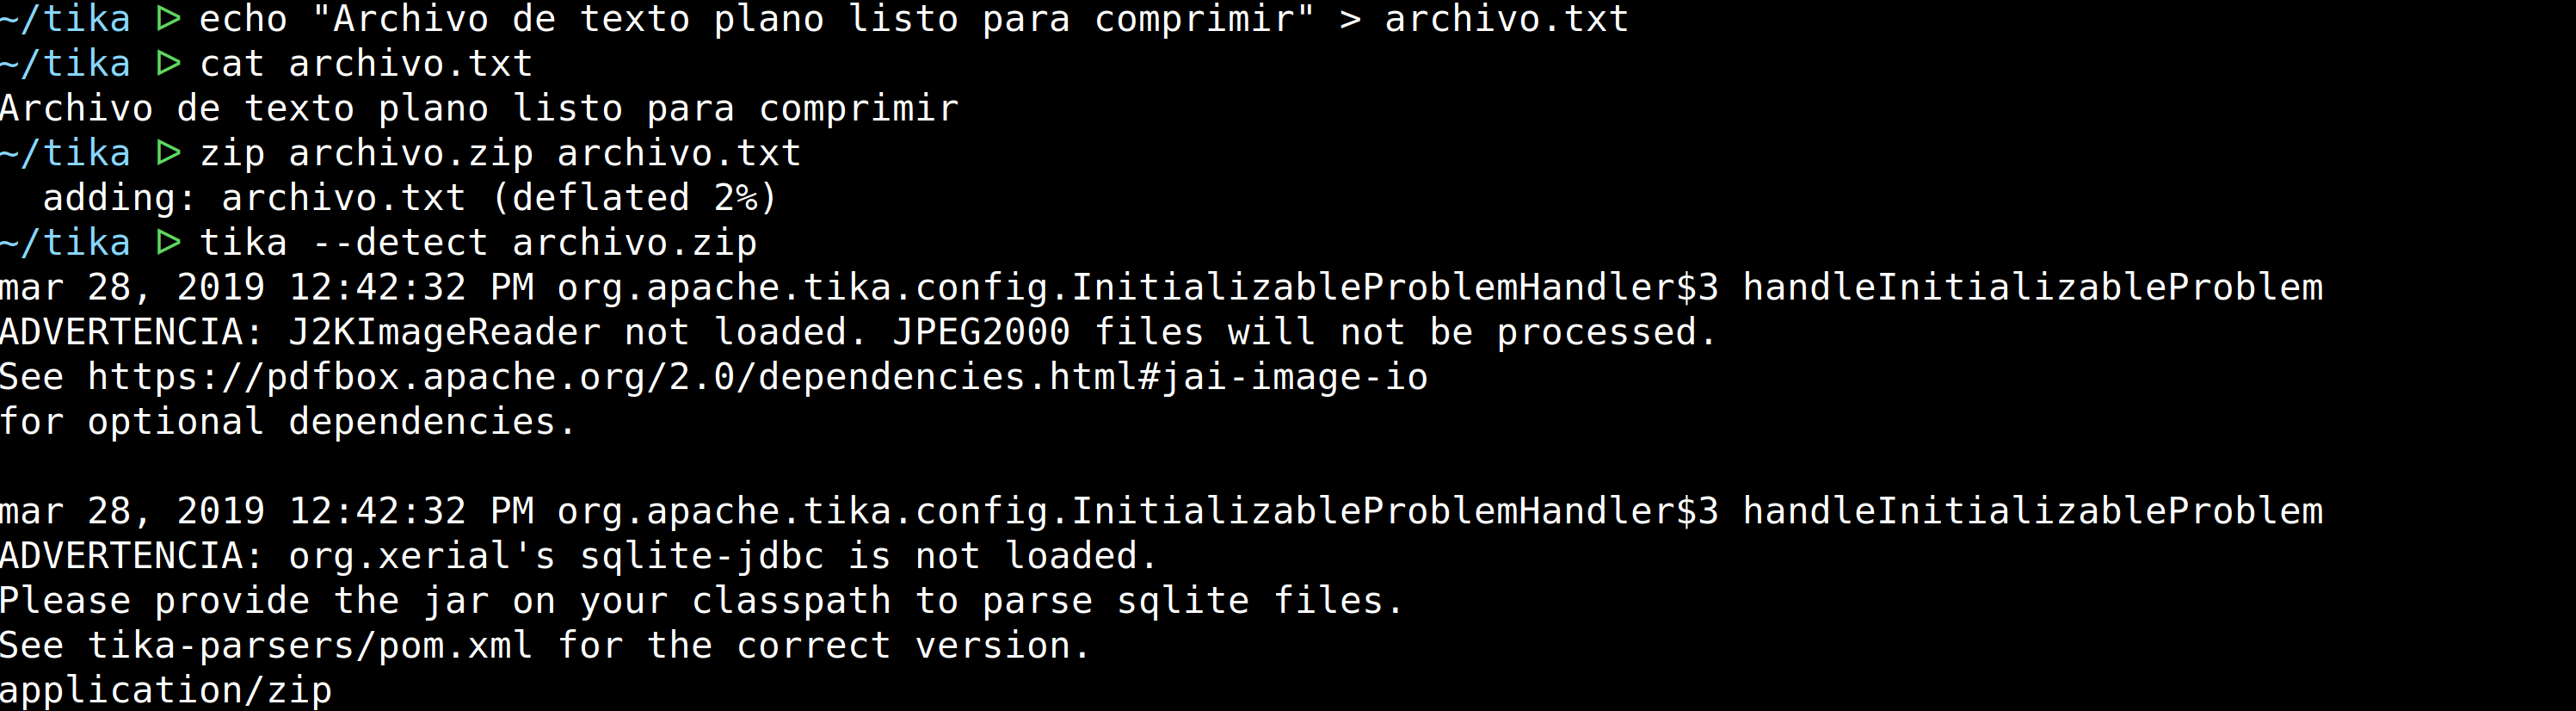
\includegraphics[width=0.7\linewidth]{./ej4}
                \caption{Ejercicio 4.}
                \end{figure}
            \item tika --metadata archivo.zip
                \begin{figure}[H]
                \centering
                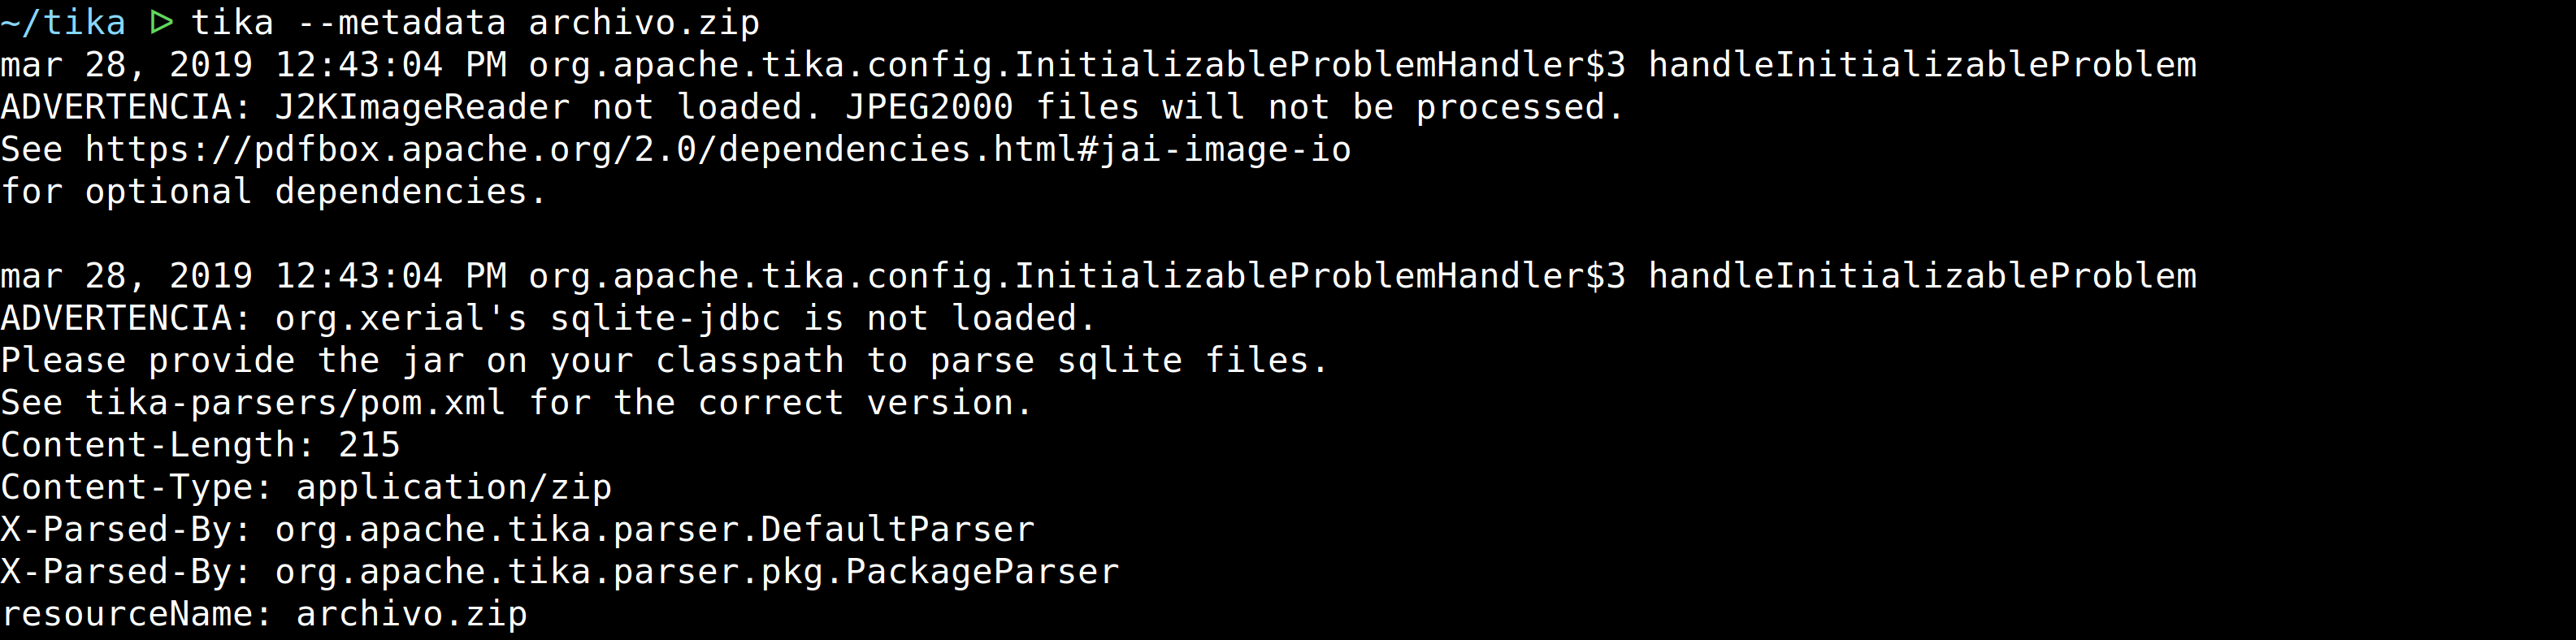
\includegraphics[width=0.7\linewidth]{./ej5}
                \caption{Ejercicio 4.}
                \end{figure}
        \end{enumerate}
    \item
        \begin{enumerate}
            \item tika --metadata ImagenCorreo.jpg
                \begin{figure}[H]
                \centering
                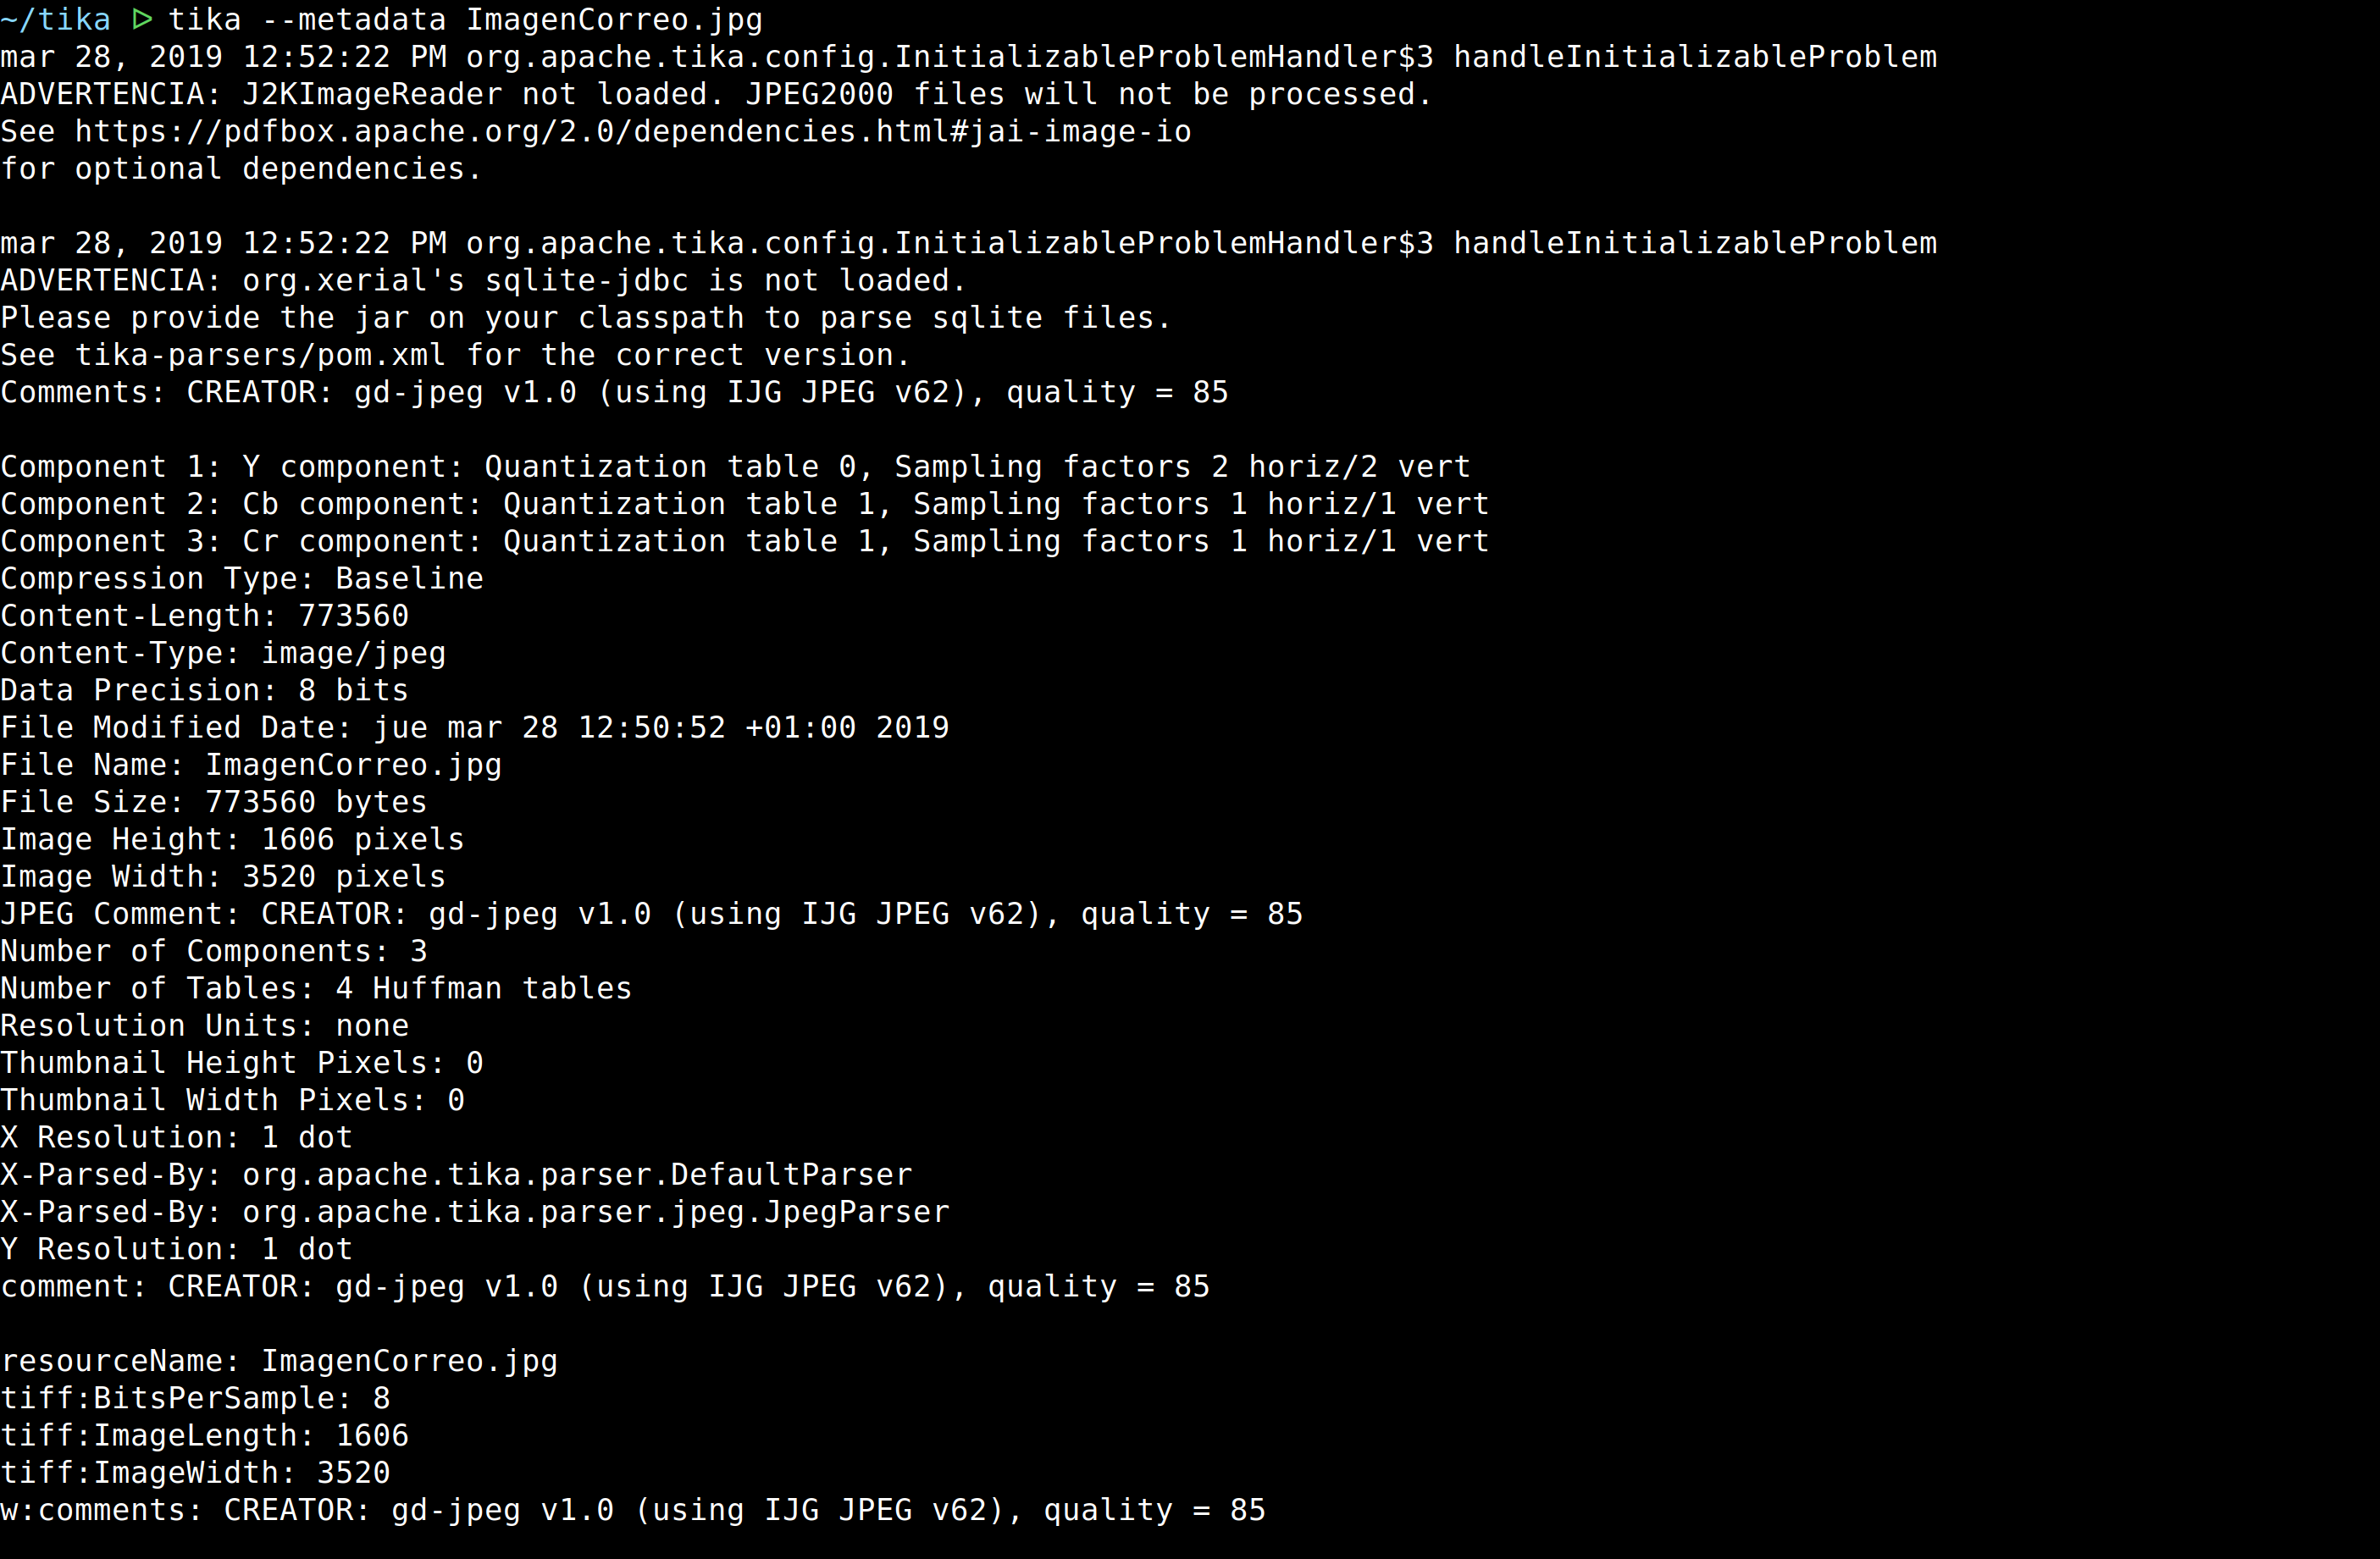
\includegraphics[width=0.7\linewidth]{./ej6}
                \caption{Ejercicio 5.}
                \end{figure}
            \item tika --metadata ImagenWhatsapp.jpeg
                \begin{figure}[H]
                \centering
                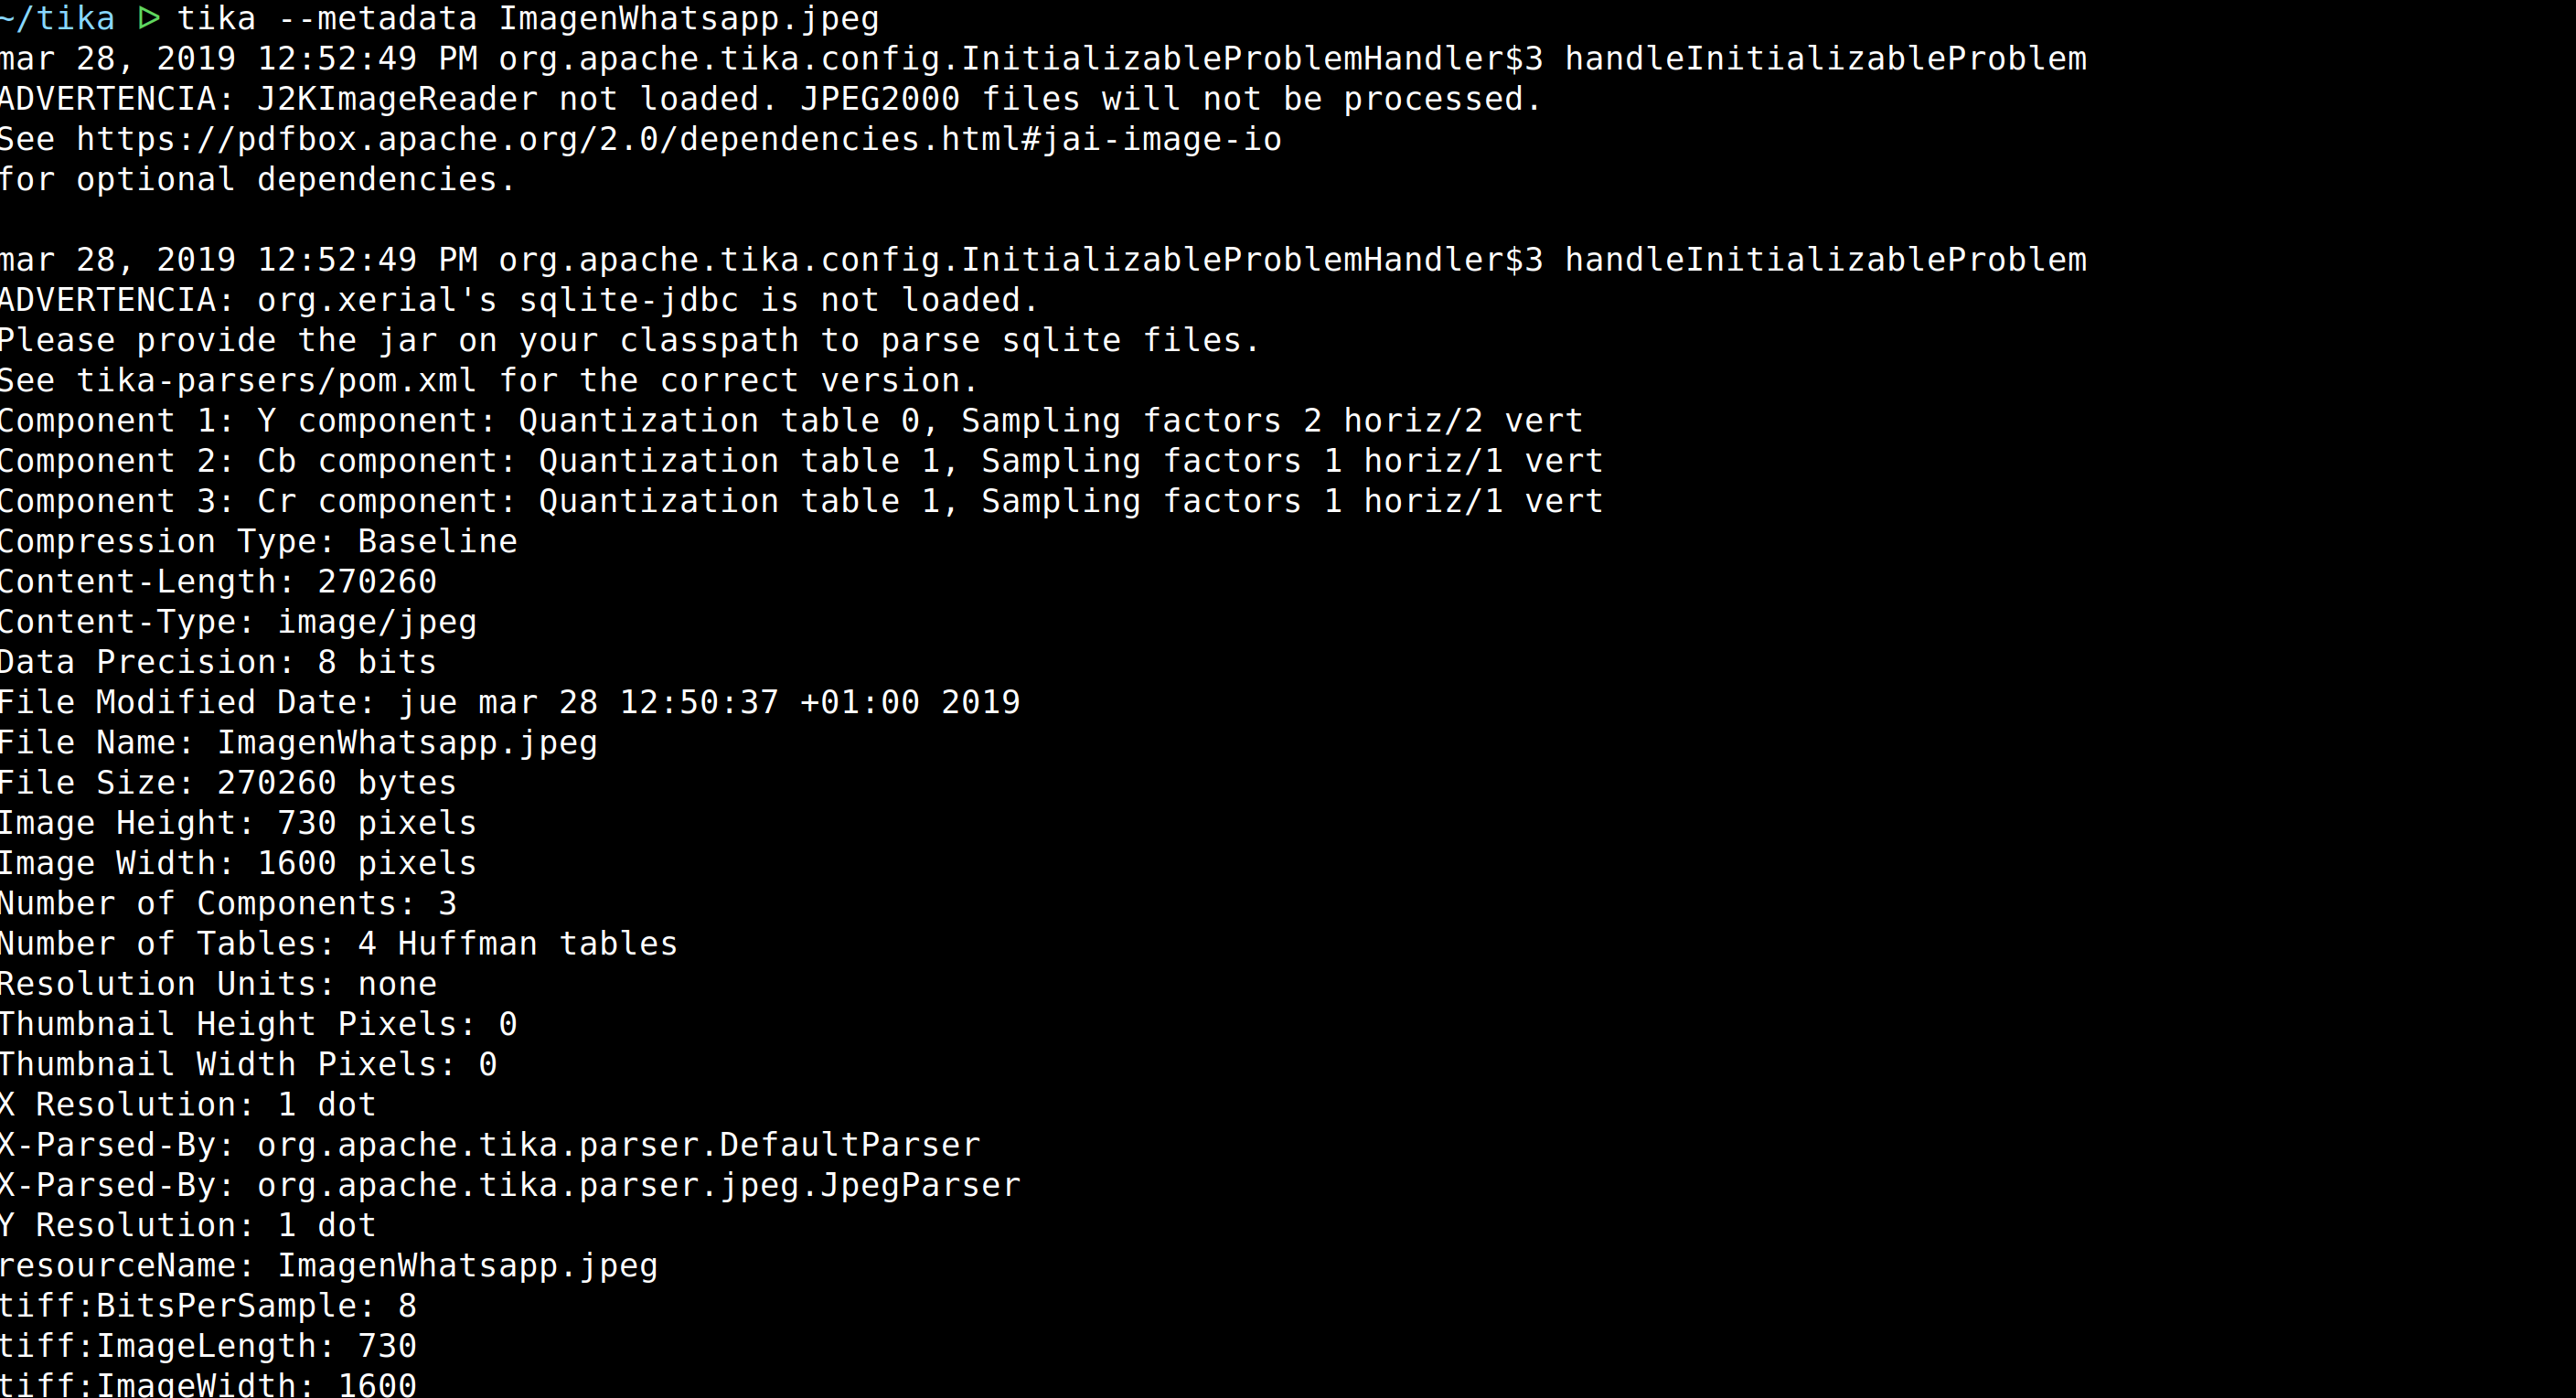
\includegraphics[width=0.7\linewidth]{./ej7}
                \caption{Ejercicio 5.}
                \end{figure}
        \end{enumerate}
    \item tika --metadata https://www.uca.es $>$ metadatosuca.txt
    \verbatiminput{metadatosuca.txt}
    \item
        \begin{enumerate}
            \item tika --text-main celebs\_fixed.rdf $>$ celebs\_fixed.doc
                \begin{figure}[H]
                \centering
                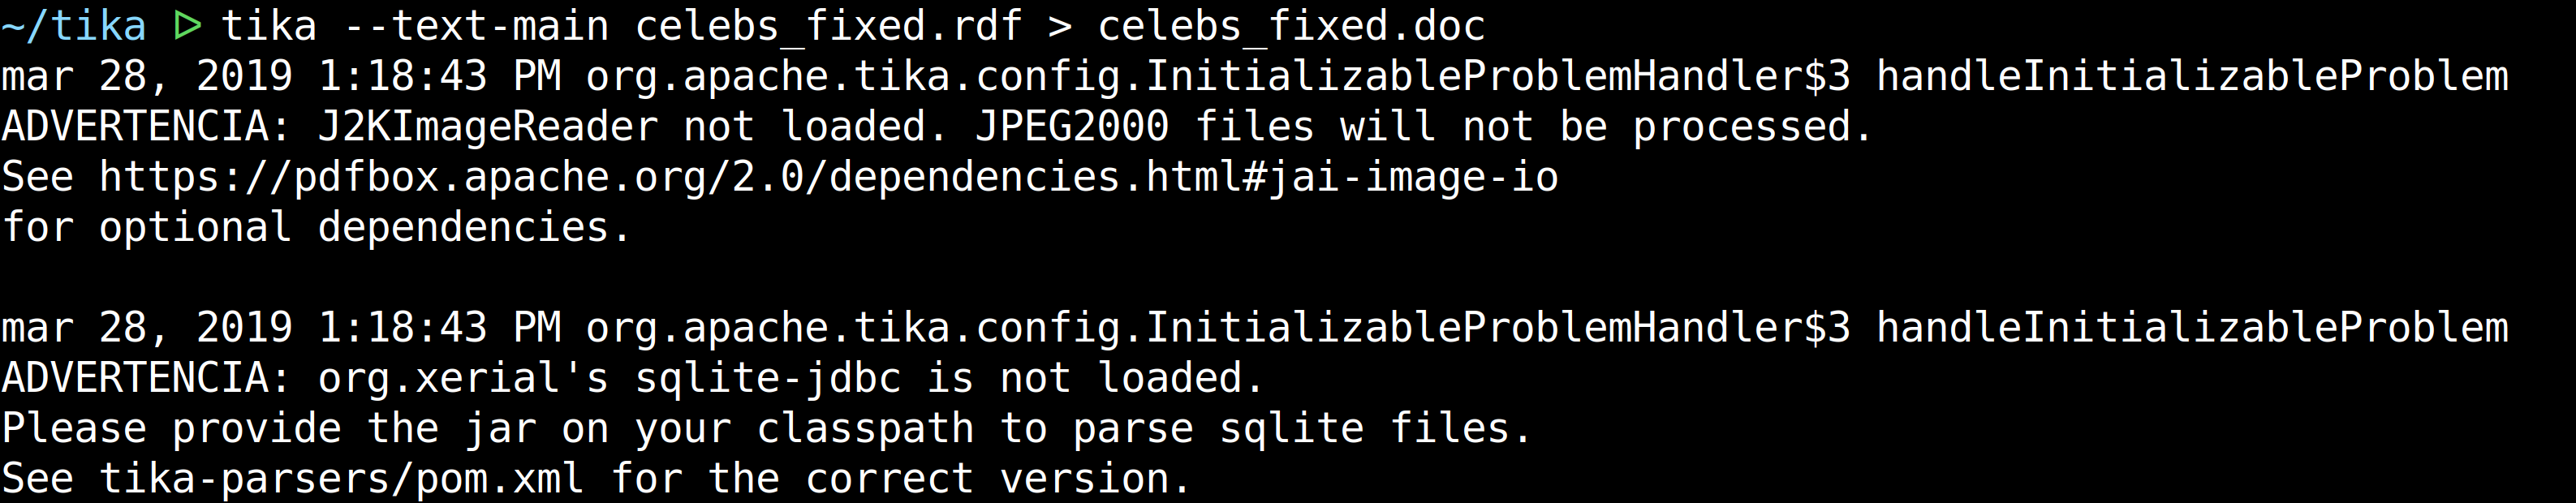
\includegraphics[width=0.7\linewidth]{./ej9}
                \caption{Ejercicio 7.}
                \end{figure}
            \item tika --text-main celebs\_fixed.rdf $>$ celebs\_fixed.pdf
                \begin{figure}[H]
                \centering
                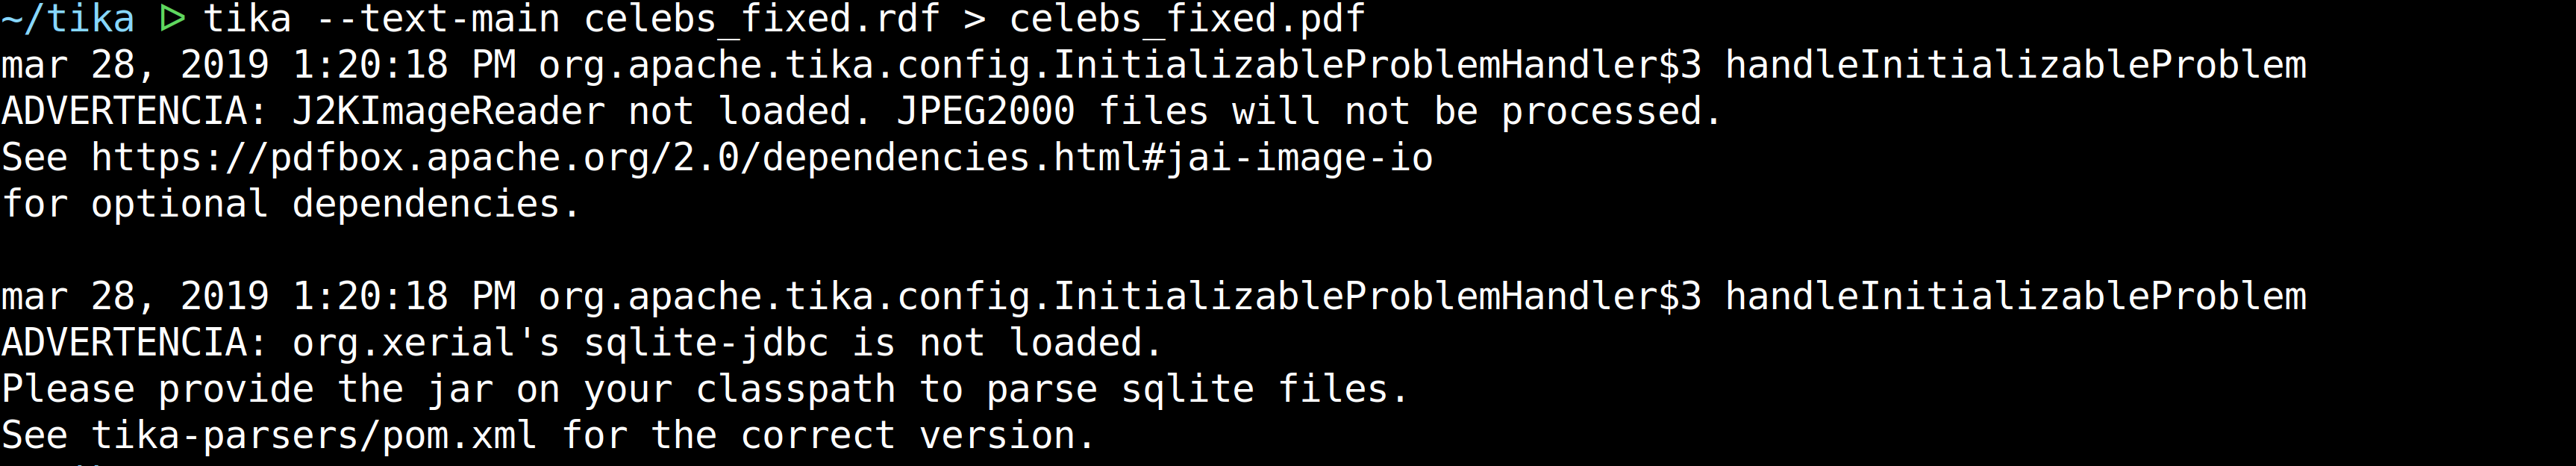
\includegraphics[width=0.7\linewidth]{./ej10}
                \caption{Ejercicio 7.}
                \end{figure}
            \item okular celebs\_fixed.pdf \&
                \begin{figure}[H]
                \centering
                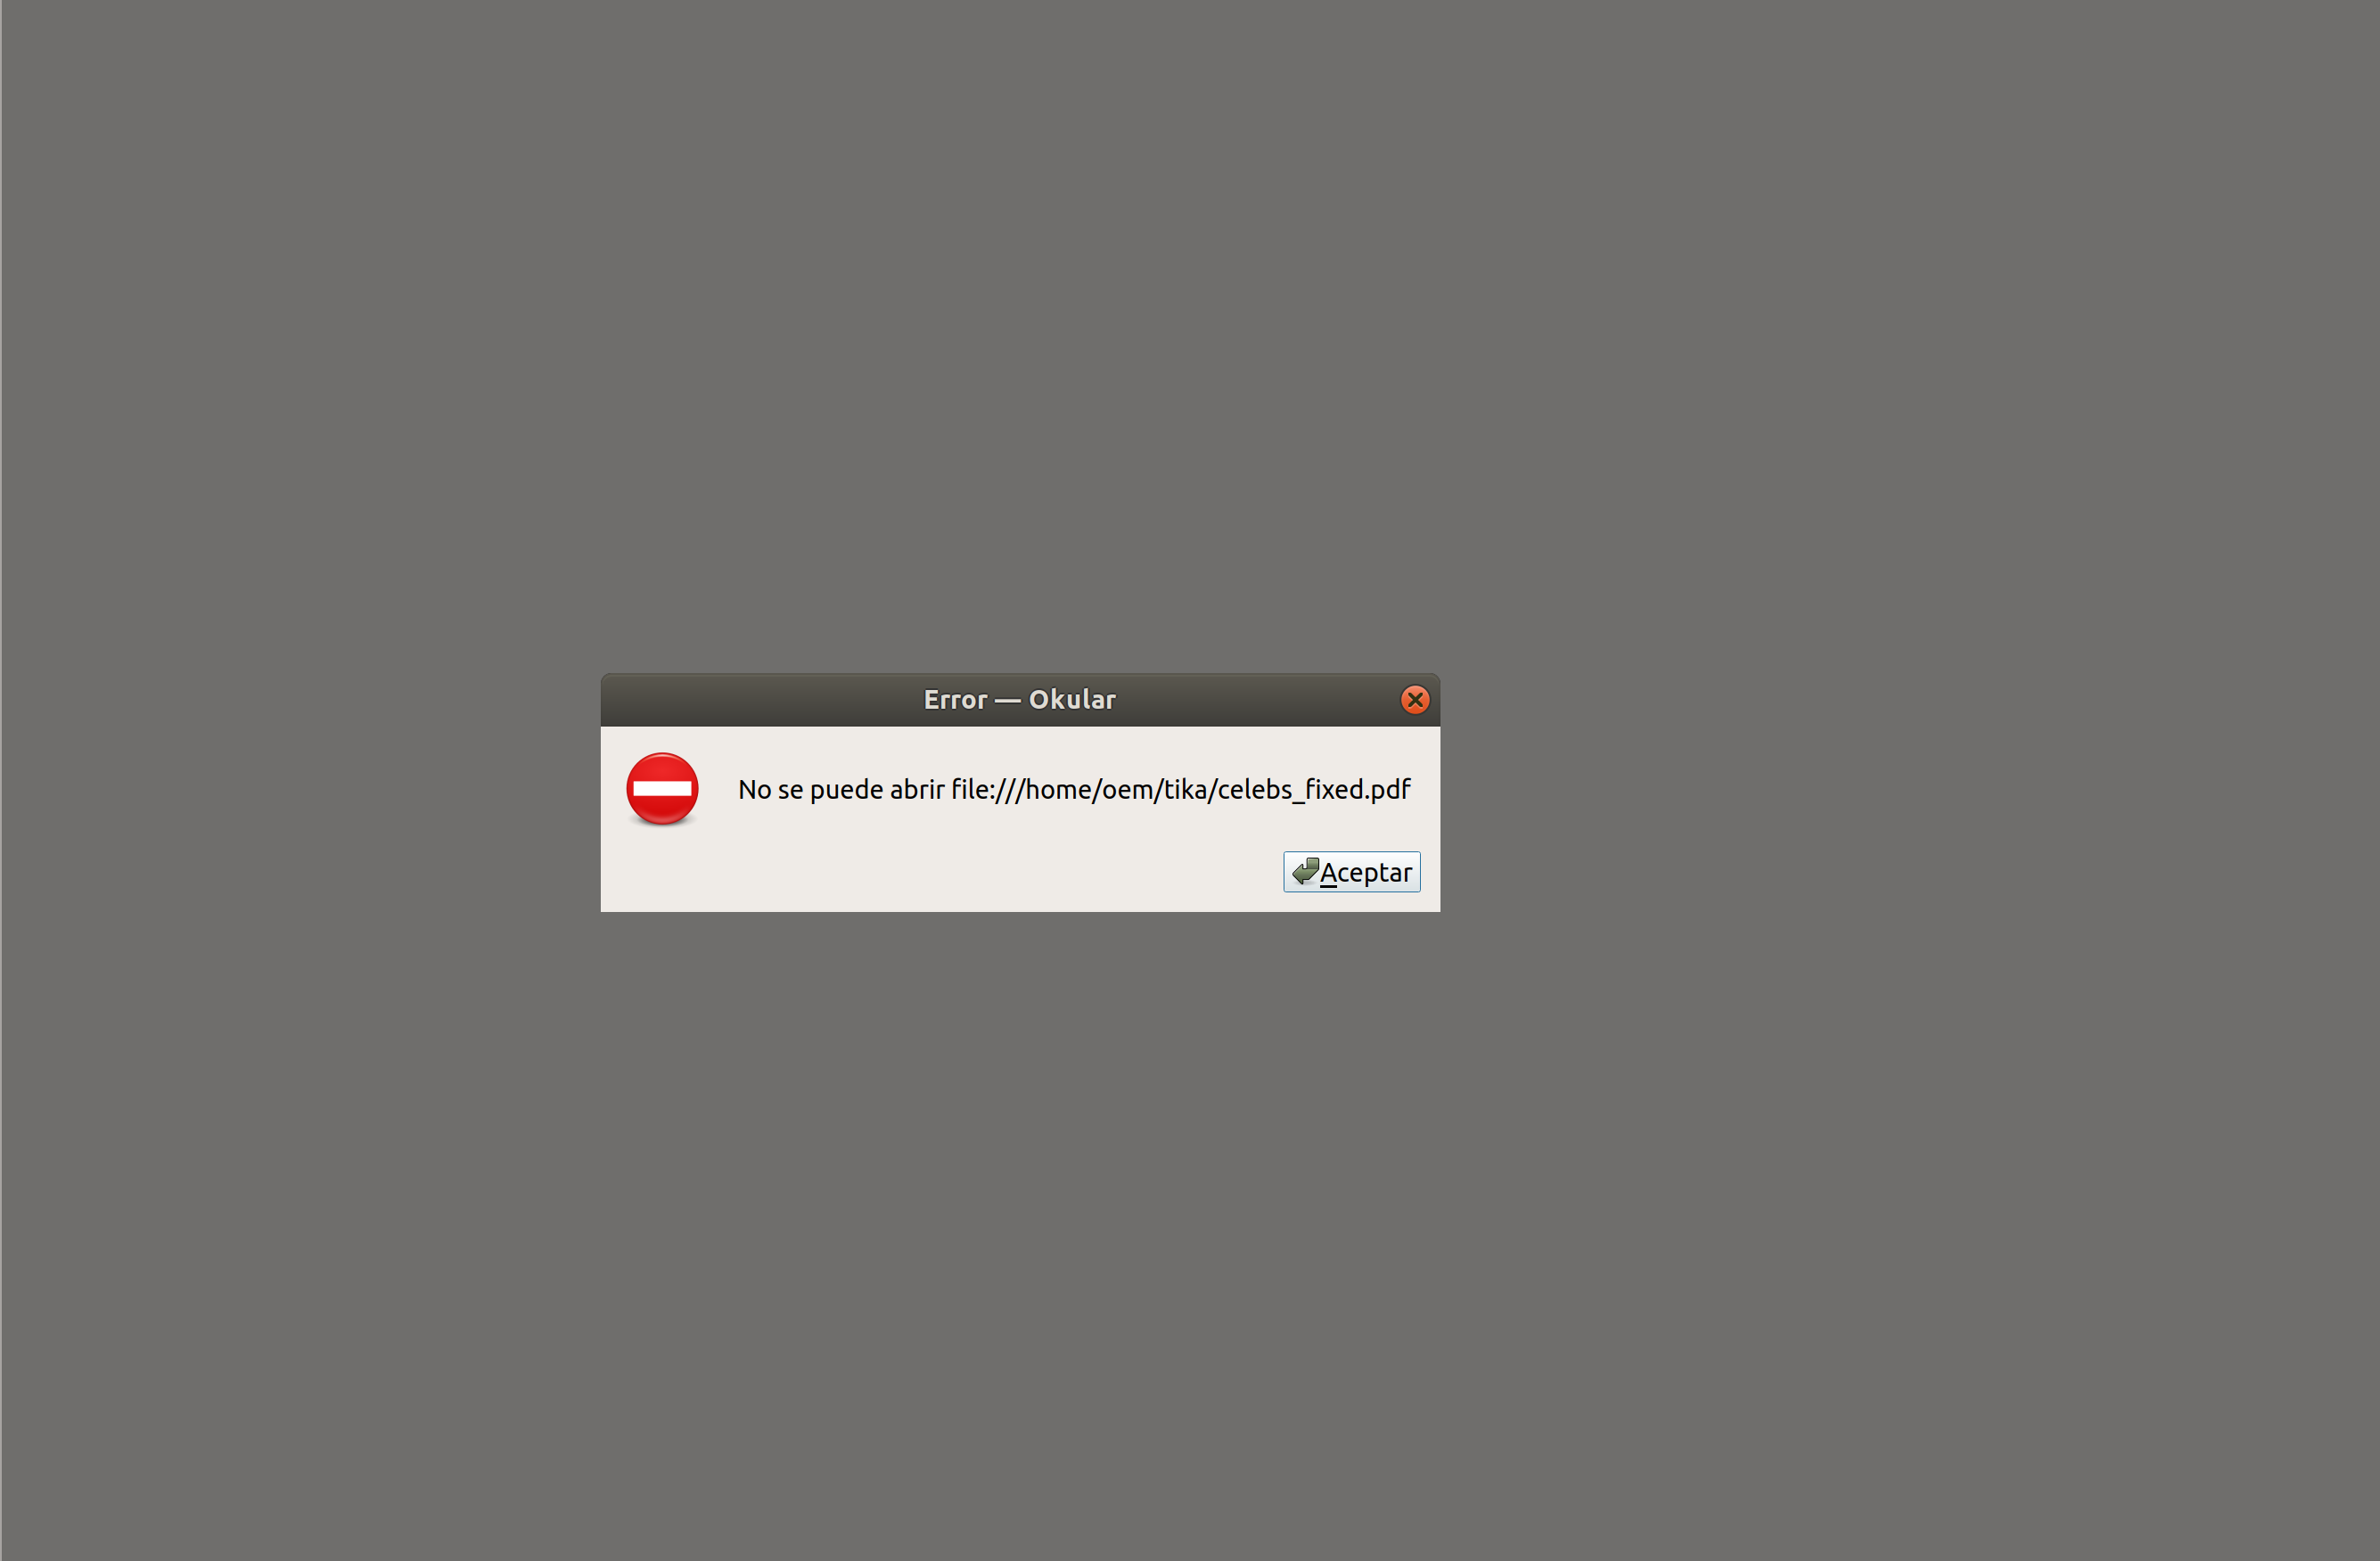
\includegraphics[width=0.7\linewidth]{./ej11}
                \caption{Ejercicio 7.}
                \end{figure}
        \end{enumerate}
    \item
        \begin{enumerate}
            \item tika --metadata q.jpg $>$ q.txt
            \item tika --metadata r.jpg $>$ q.txt
            \item tika --metadata s.JPG $>$ q.txt
        \end{enumerate}
        \begin{figure}[H]
        \centering
        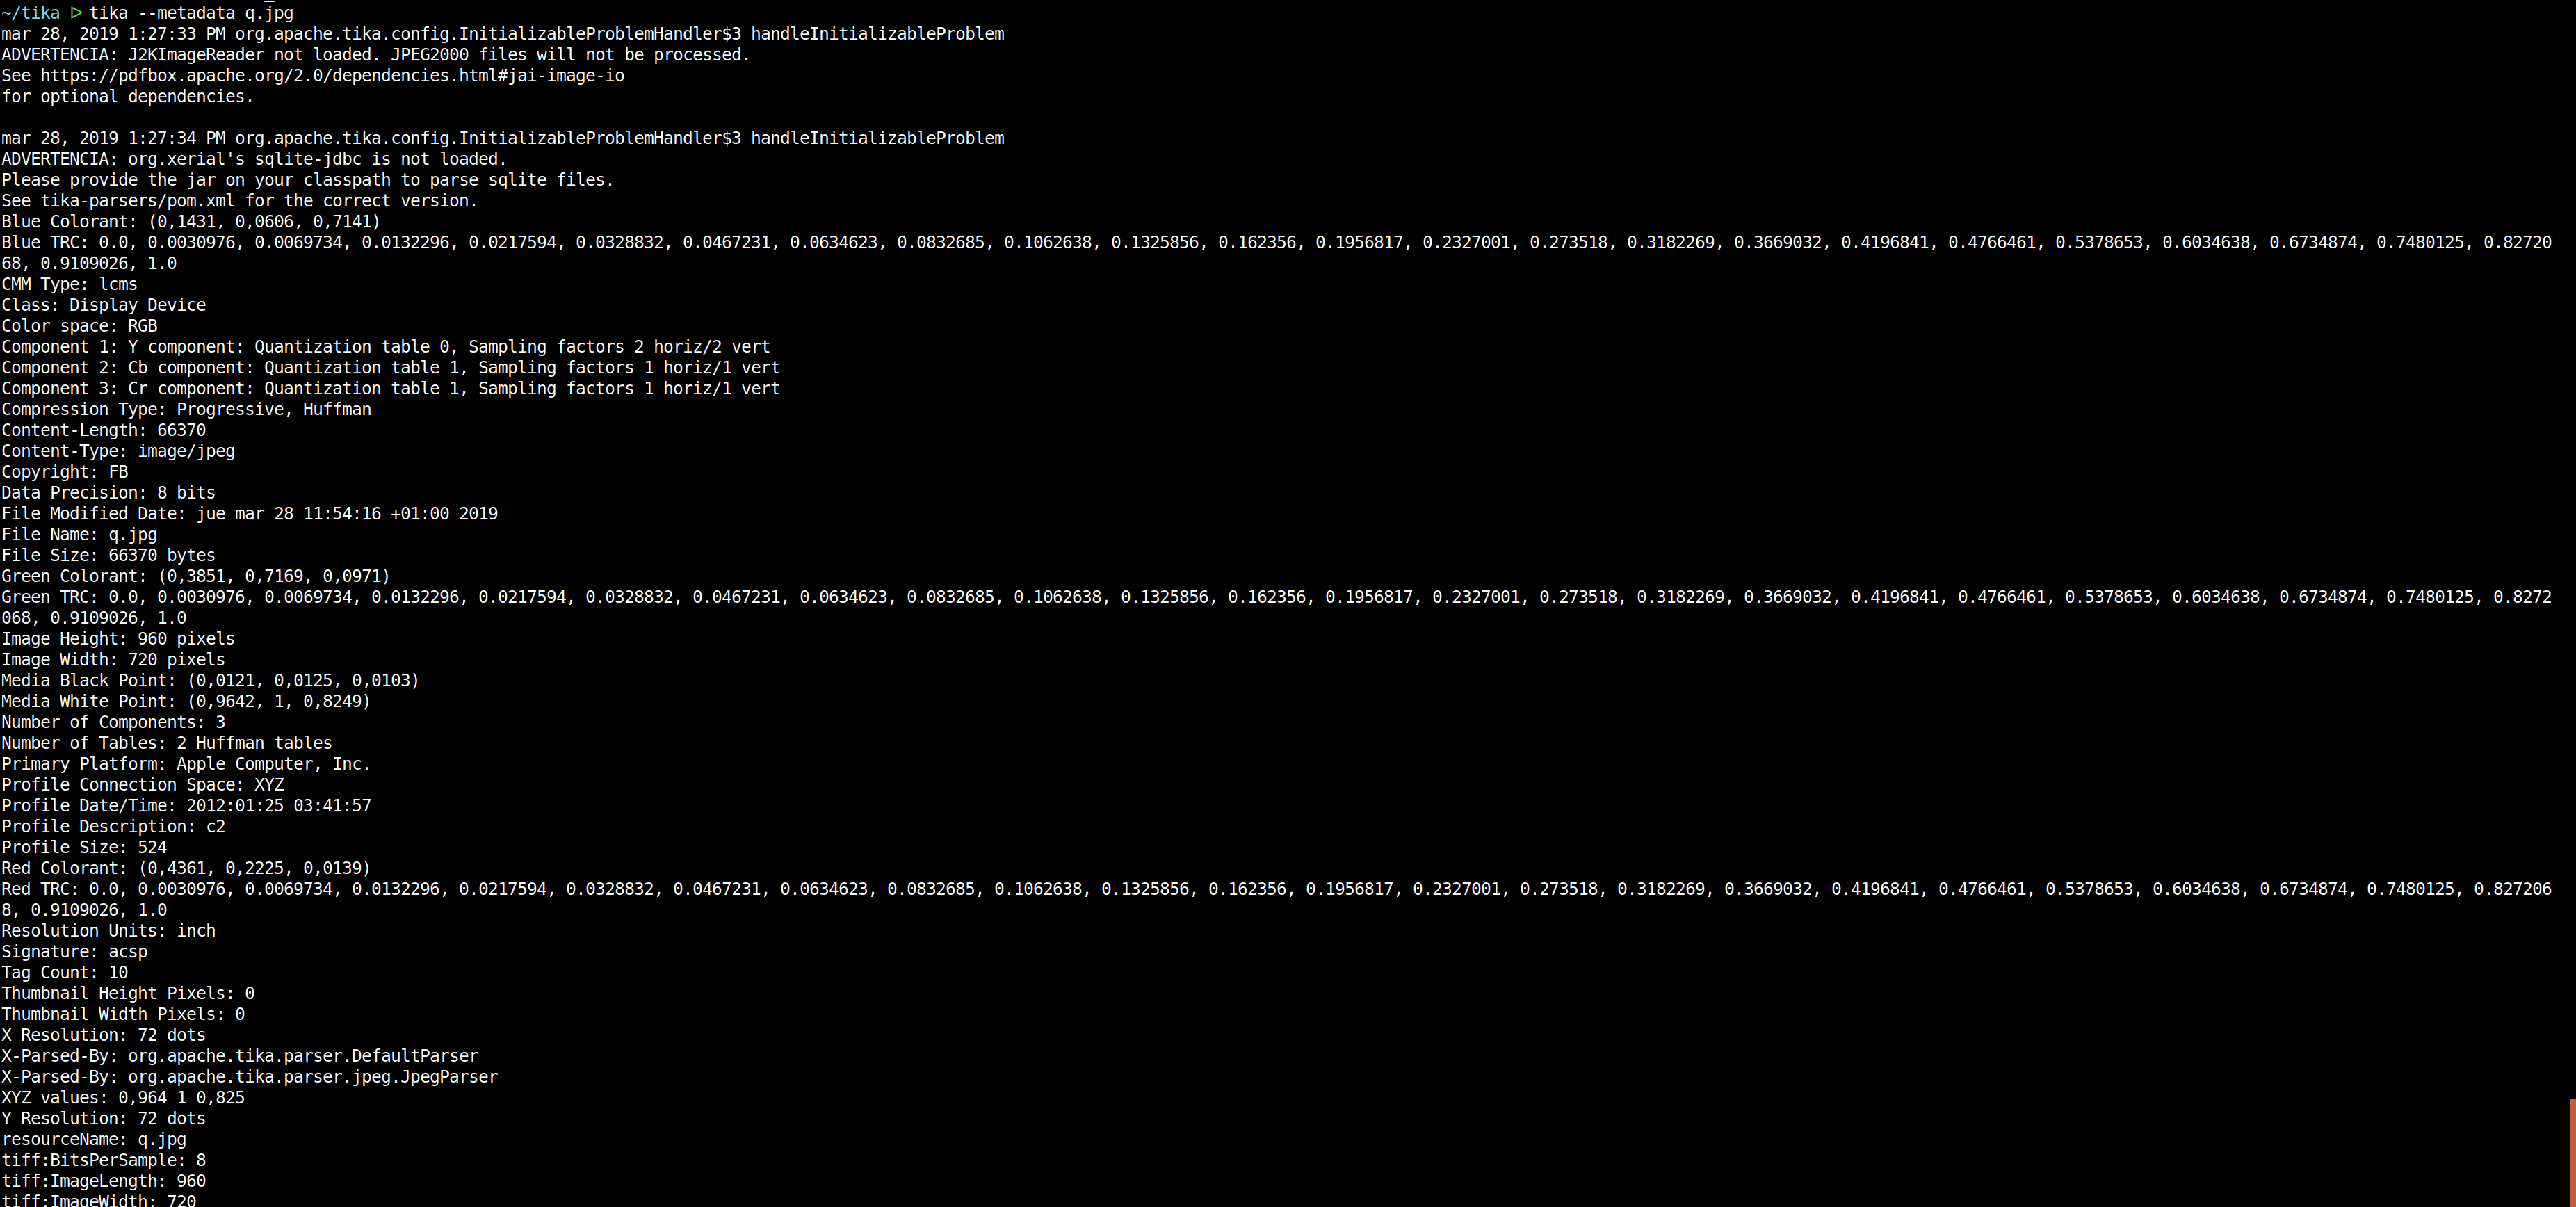
\includegraphics[width=0.7\linewidth]{./ej12}
        \caption{Ejercicio 8.}
        \end{figure}
        \begin{figure}[H]
        \centering
        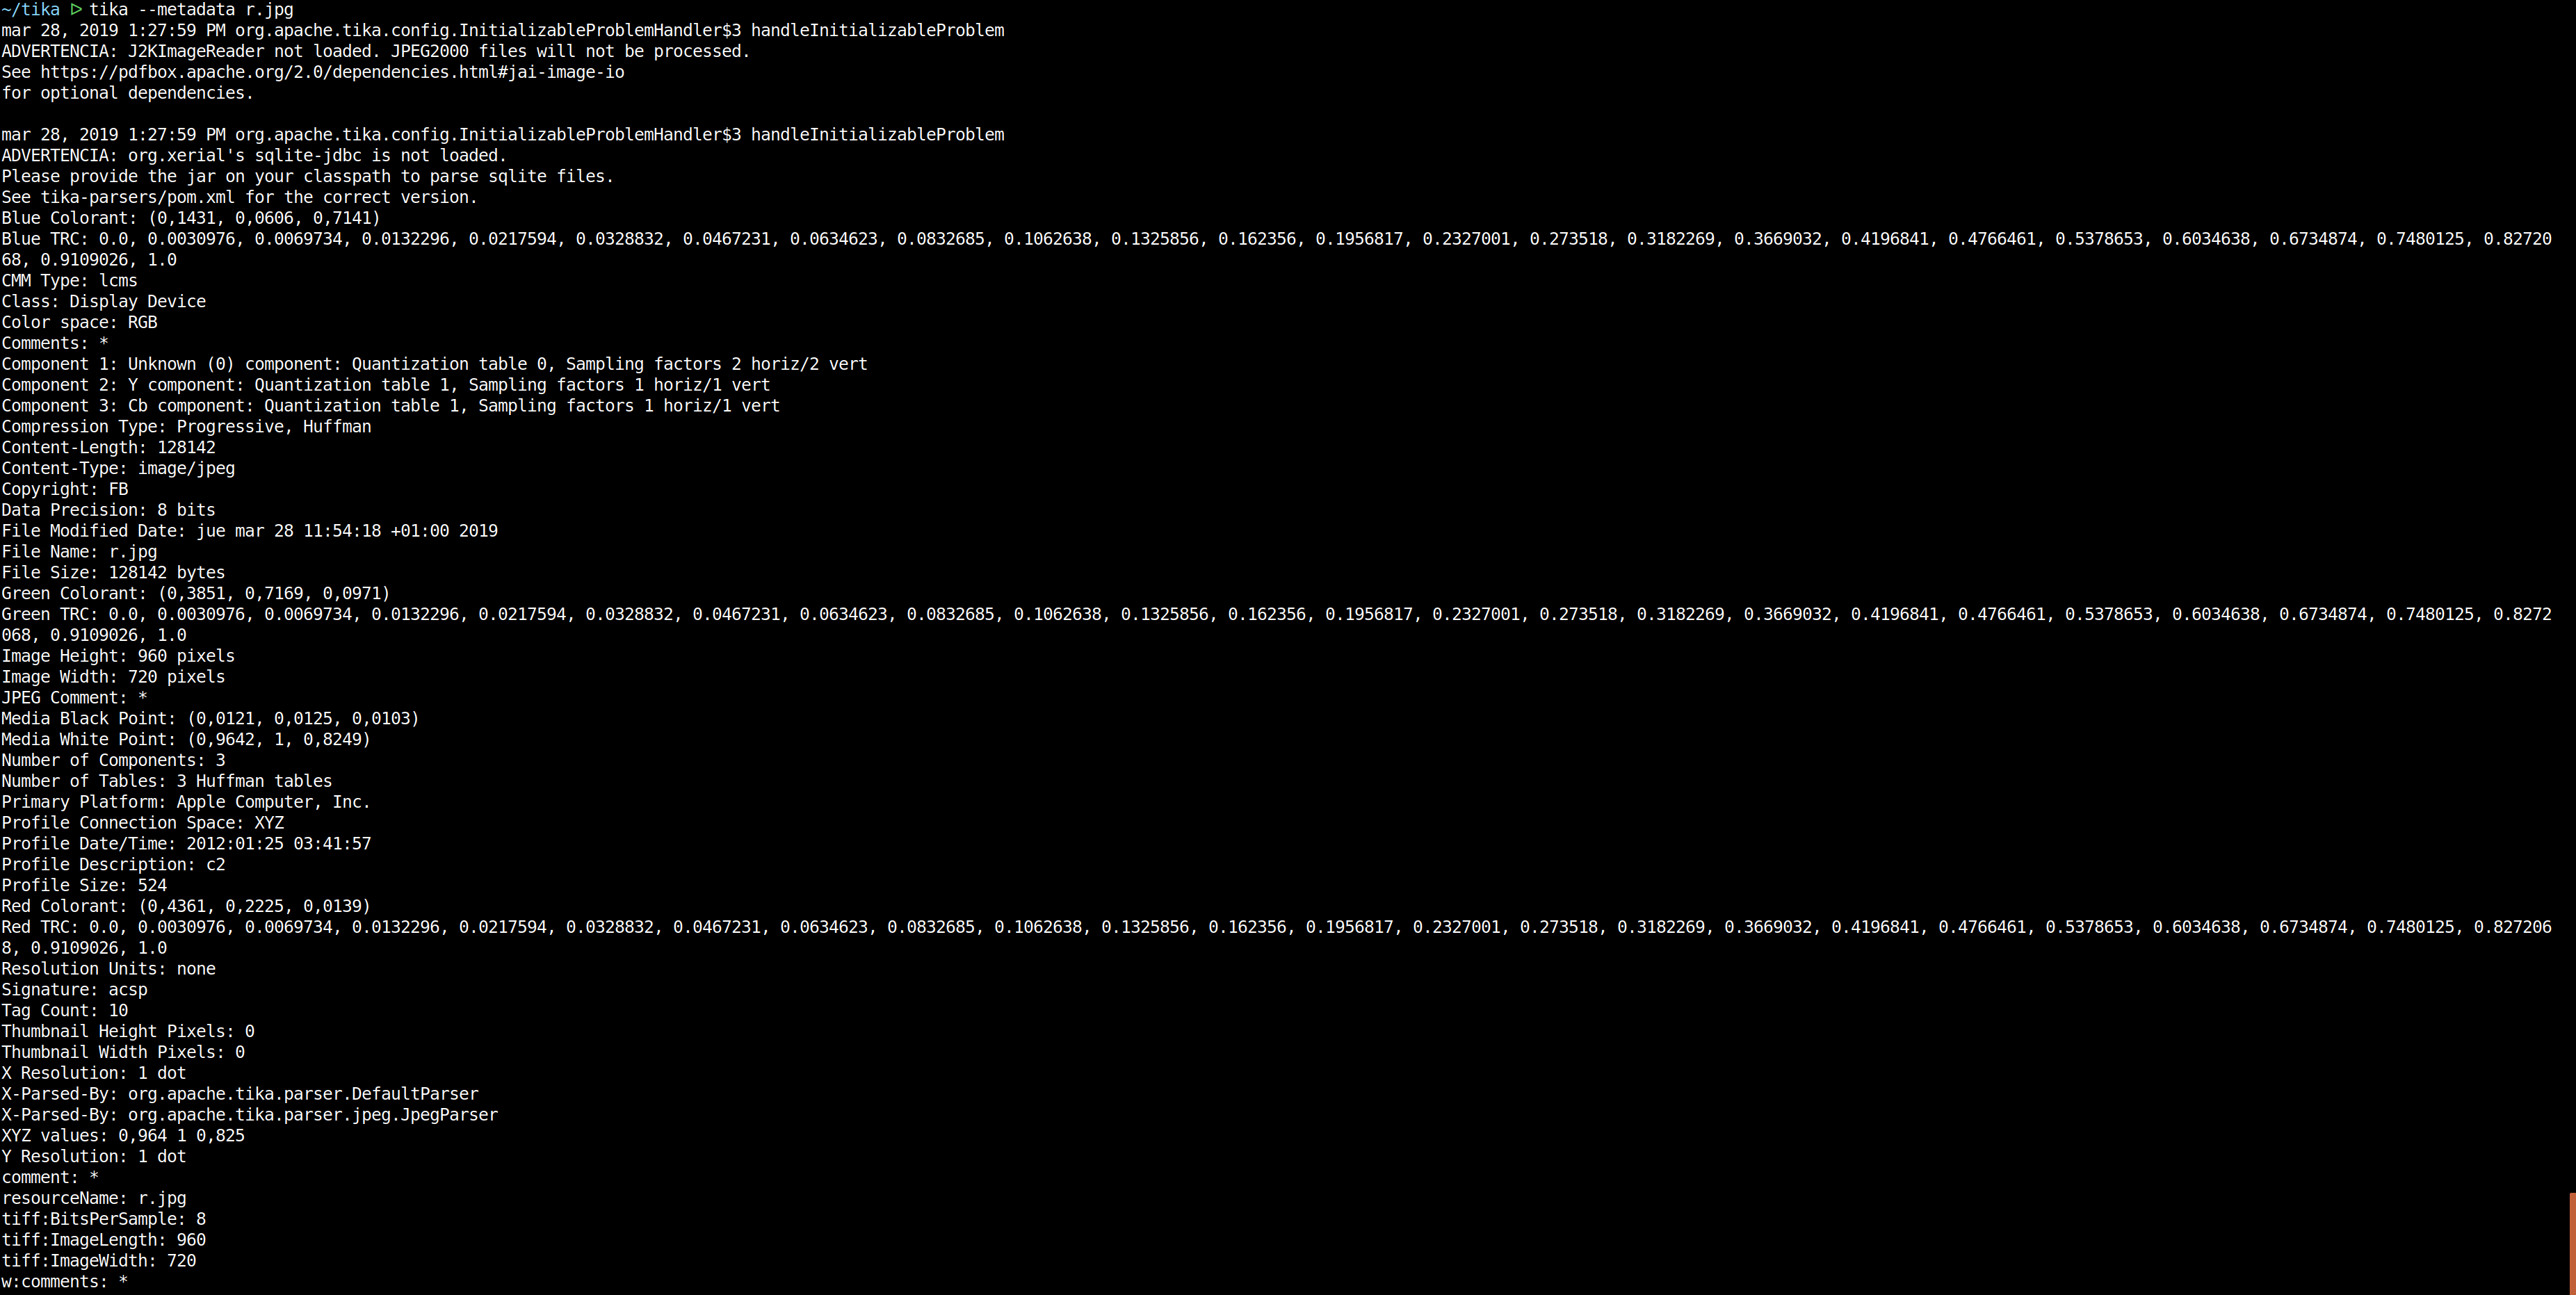
\includegraphics[width=0.7\linewidth]{./ej13}
        \caption{Ejercicio 8.}
        \end{figure}
    \item
        \begin{enumerate}
            \item tika --html https://www.uca.es $>$ uca.html
                \begin{figure}[H]
                \centering
                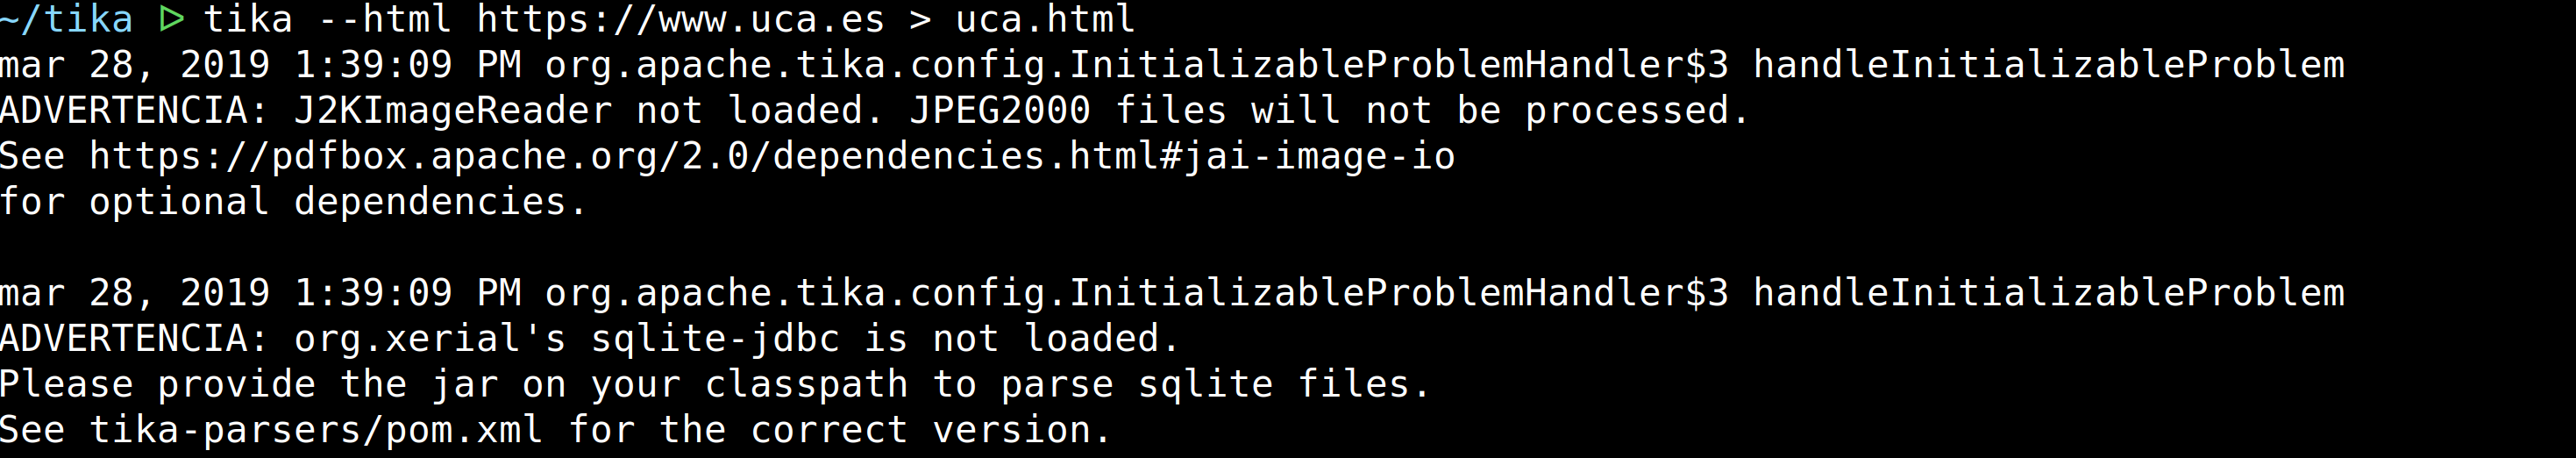
\includegraphics[width=0.7\linewidth]{./ej14}
                \caption{Ejercicio 9.}
                \end{figure}
            \item tika --html uca.html $>$ uca.doc
                \begin{figure}[H]
                \centering
                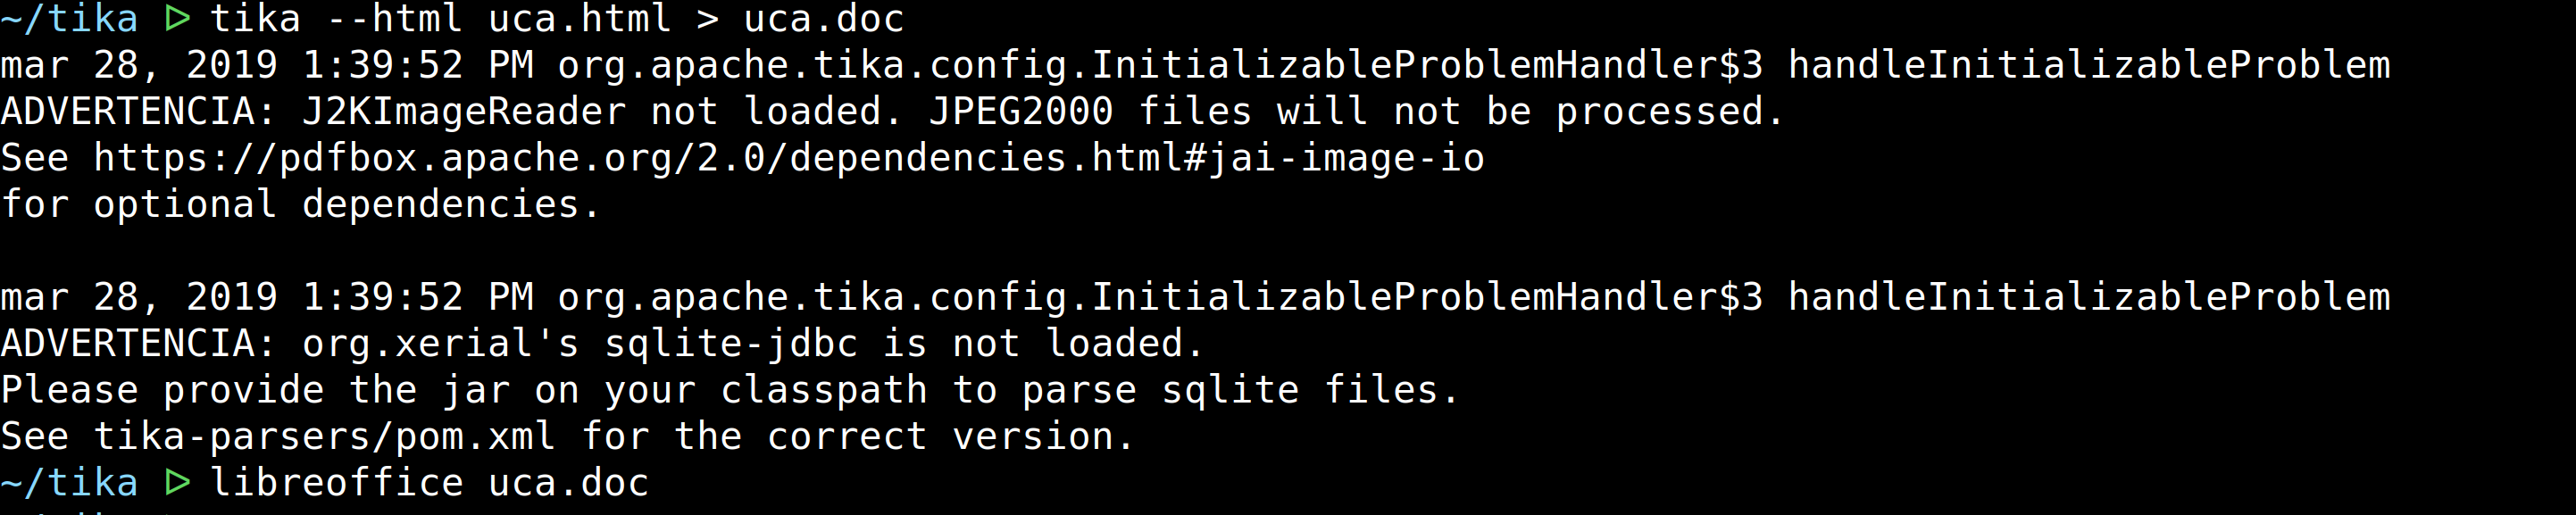
\includegraphics[width=0.7\linewidth]{./ej15}
                \caption{Ejercicio 9.}
                \end{figure}
            \item tika --metadata uca.doc
                \begin{figure}[H]
                \centering
                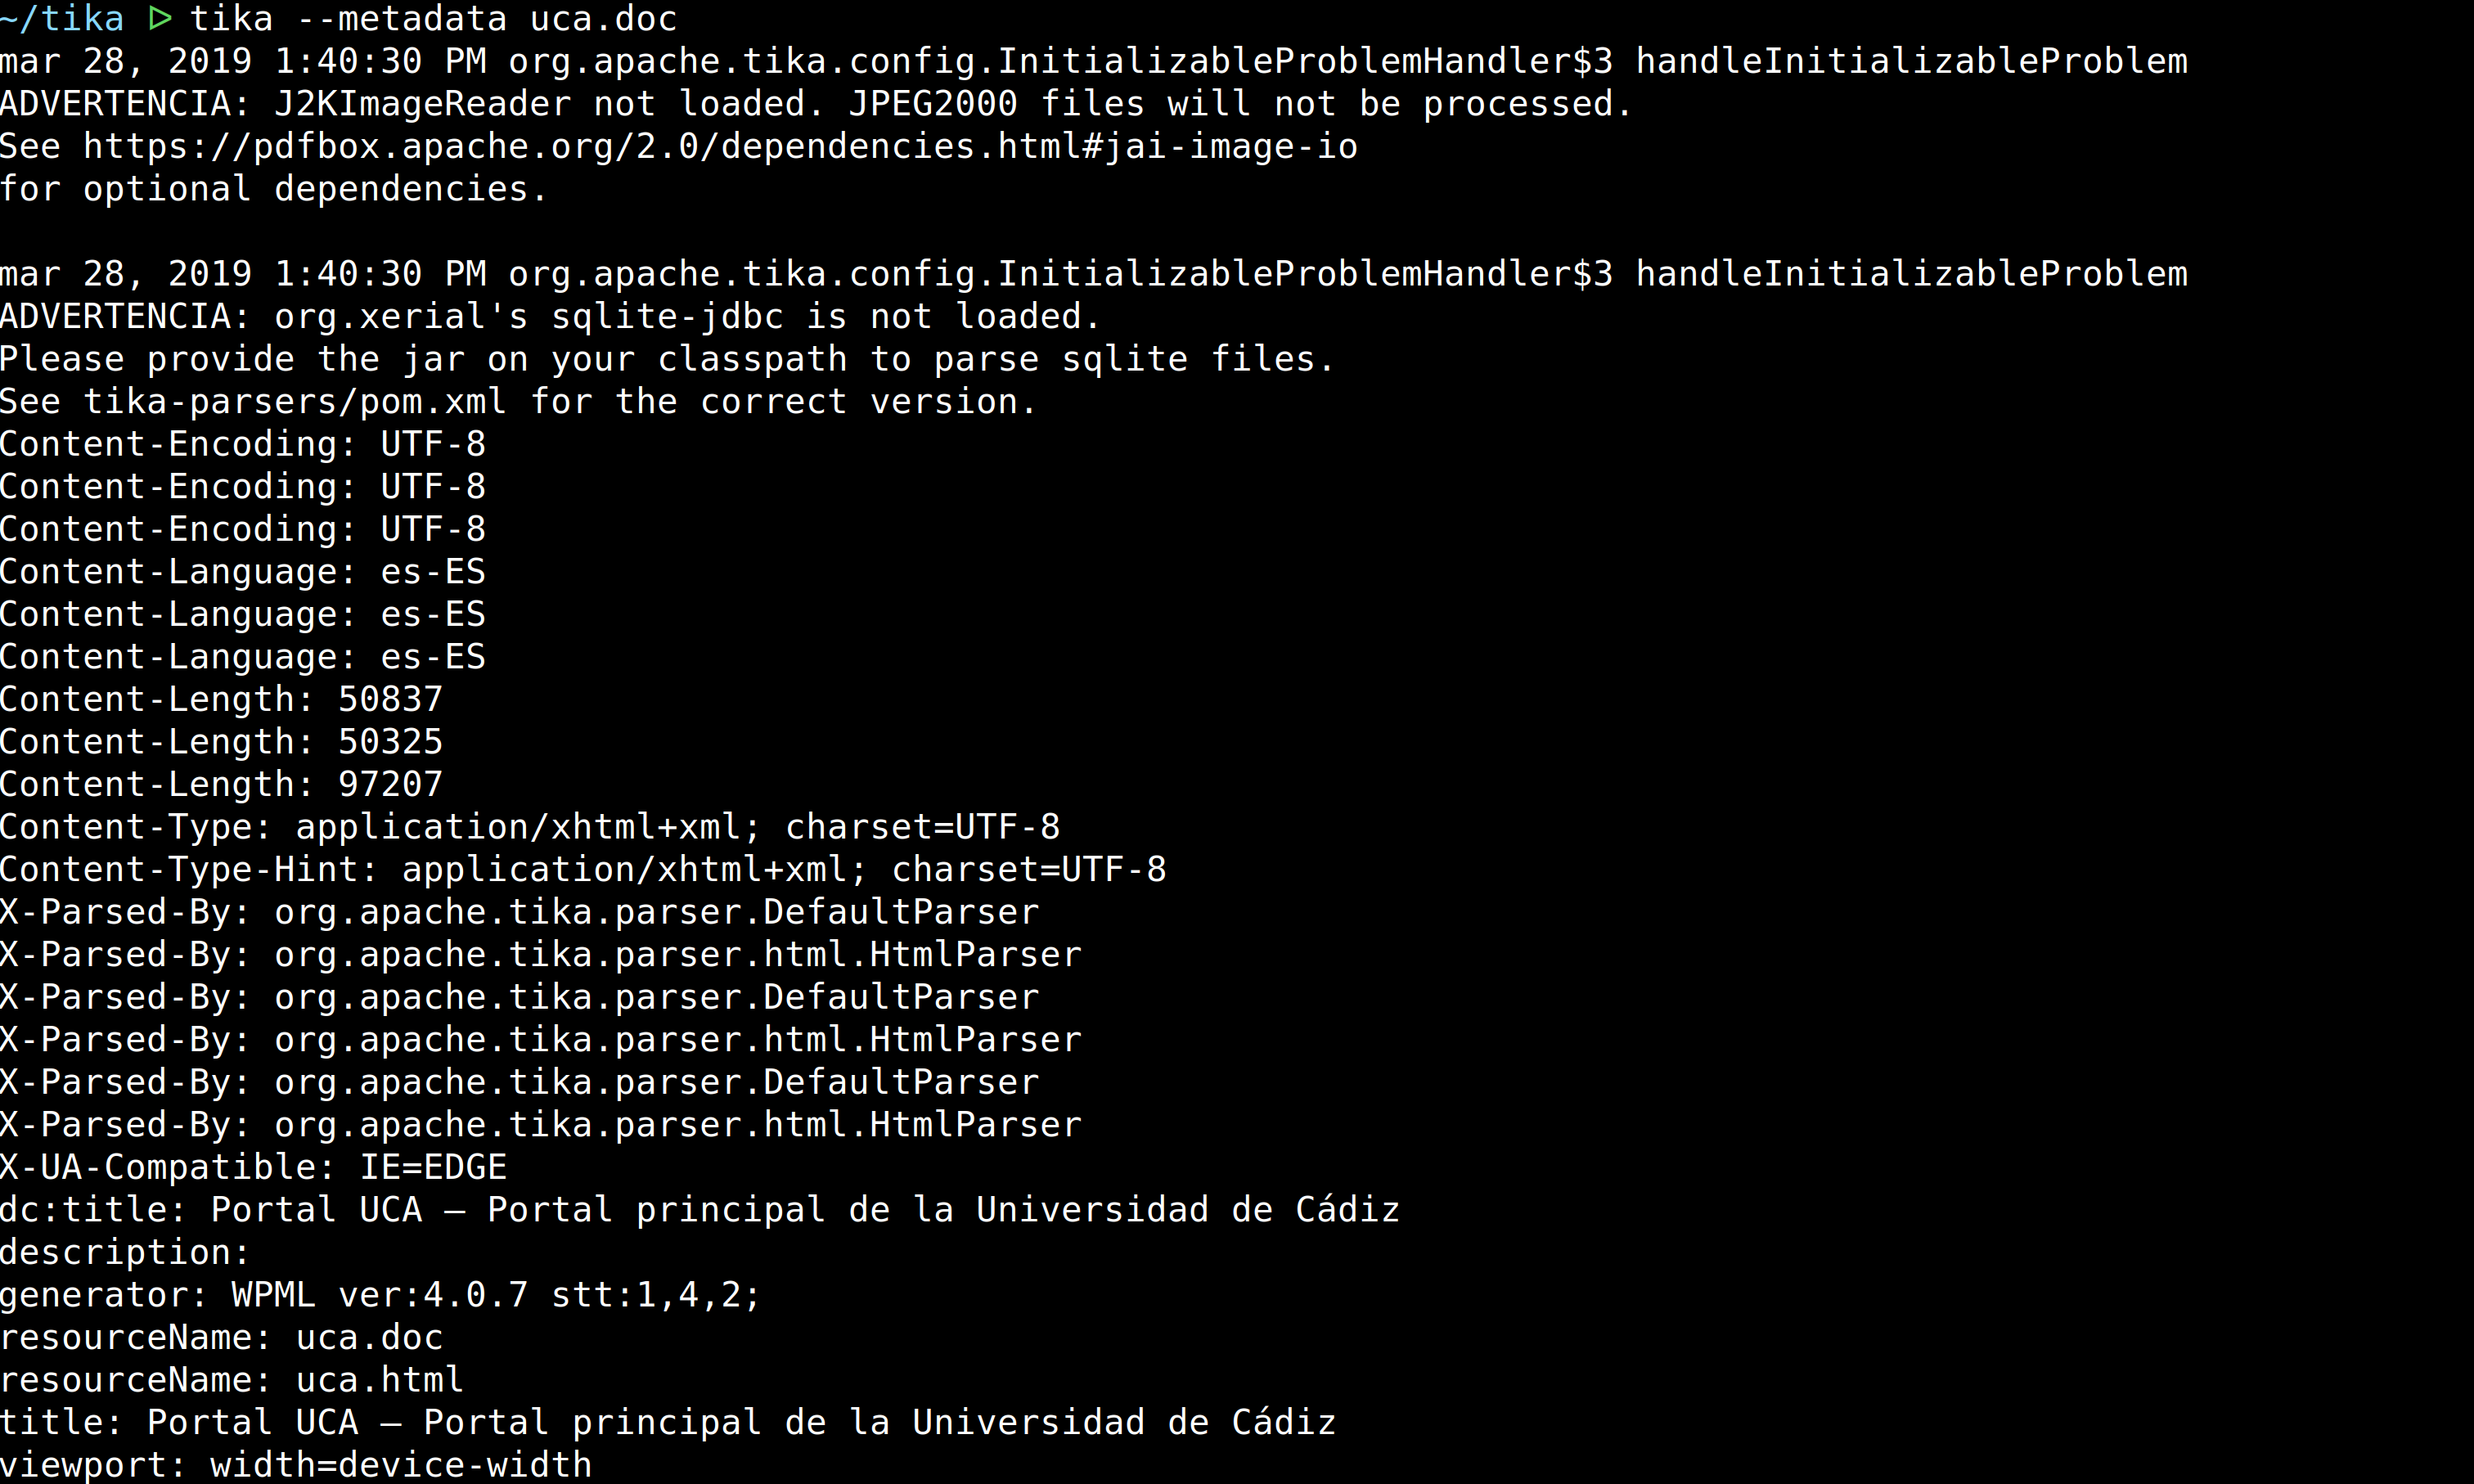
\includegraphics[width=0.7\linewidth]{./ej16}
                \caption{Ejercicio 9.}
                \end{figure}
        \end{enumerate}
    \item
        \begin{enumerate}
            \item tika --metadata primera.jpg $>$ primera.txt
                \begin{figure}[H]
                \centering
                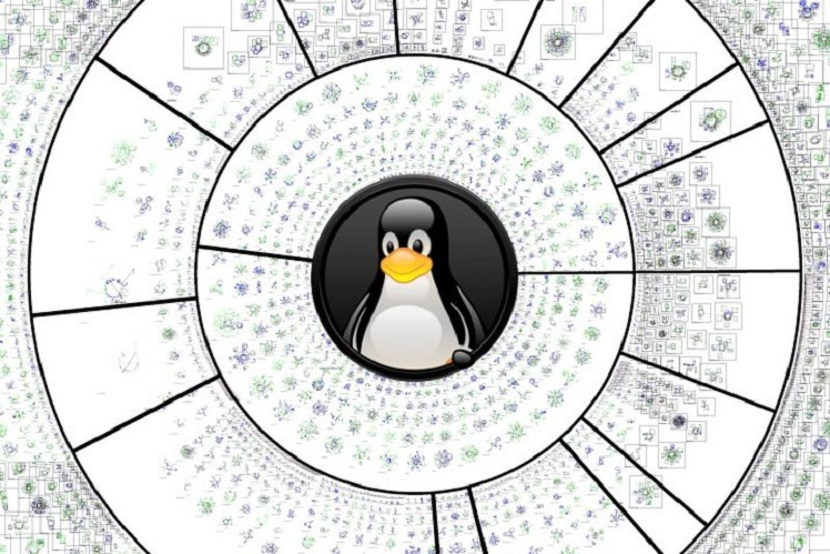
\includegraphics[width=0.7\linewidth]{./primera}
                \caption{Ejercicio 10.}
                \end{figure}
                \verbatiminput{primera.txt}
            \item tika --metadata segunda.png $>$ segunda.txt
                \begin{figure}[H]
                \centering
                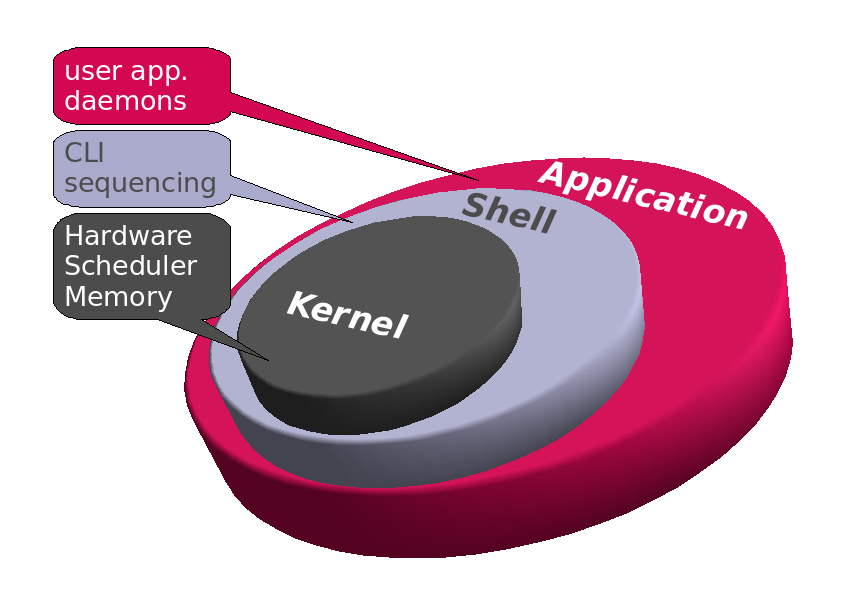
\includegraphics[width=0.7\linewidth]{./segunda}
                \caption{Ejercicio 10.}
                \end{figure}
                \verbatiminput{primera.txt}
            \item tika --metadata tercera.png $>$ tercera.txt
                \begin{figure}[H]
                \centering
                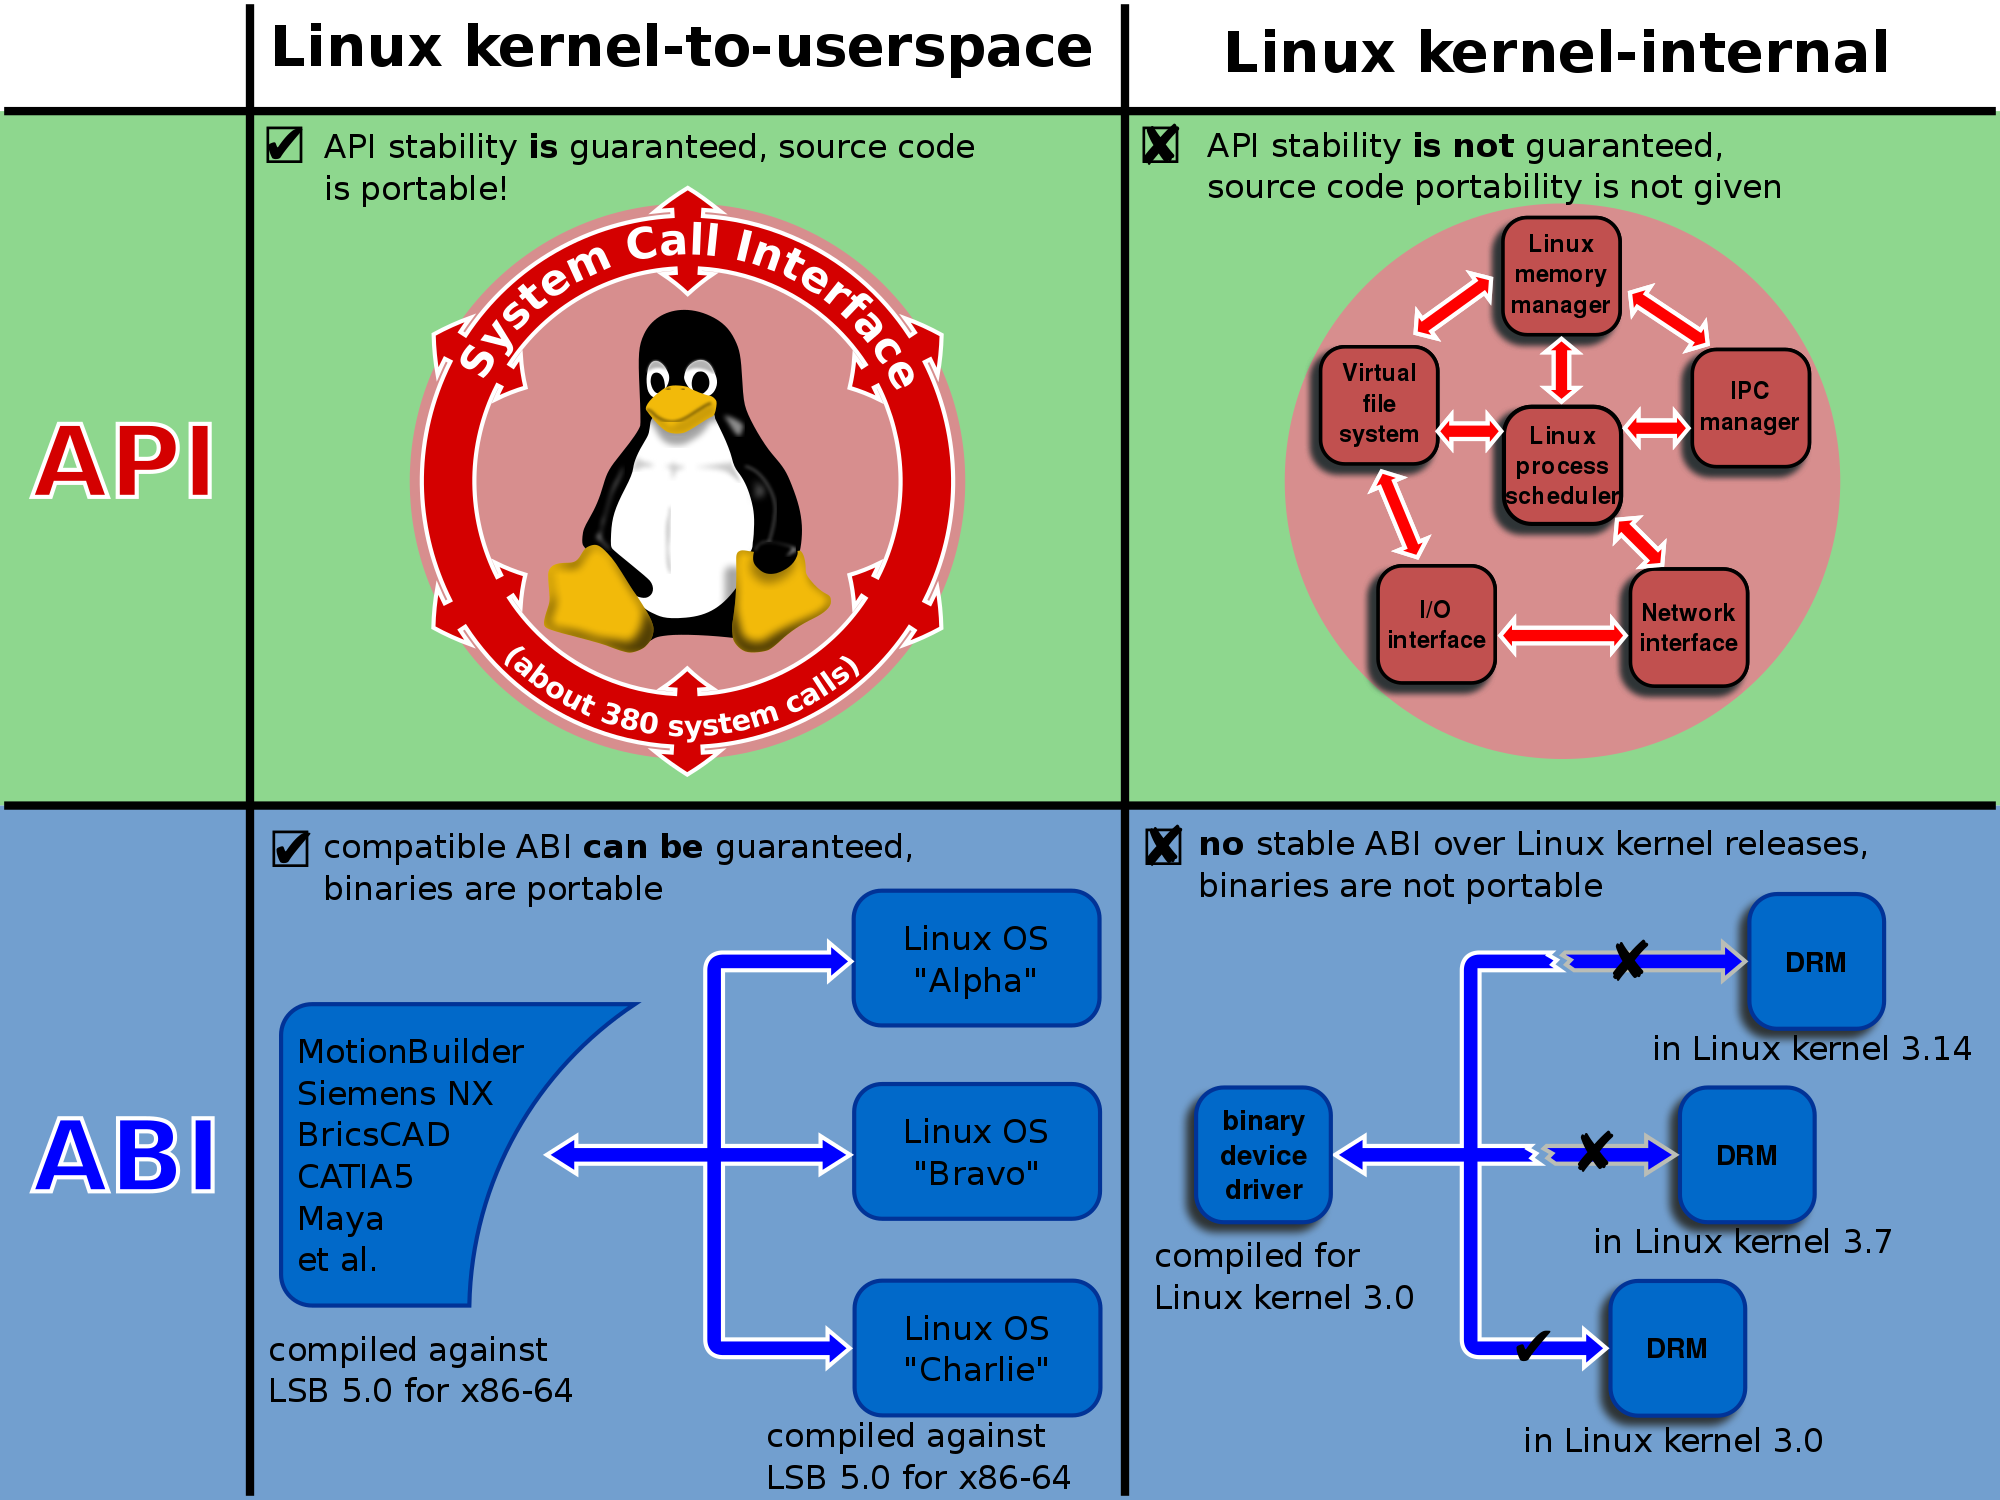
\includegraphics[width=0.7\linewidth]{./tercera}
                \caption{Ejercicio 10.}
                \end{figure}
                \verbatiminput{primera.txt}
        \end{enumerate}
    \item Los pasos a seguir son:
        \begin{enumerate}
            \item Instalar eclipse.
            \item Crear un proyecto en Java con eclipse.
            \item Ir a la zona de `Project $>$ Properties $>$ Java Build Paths $>$ Libraries $>$ Add External JARS\ldots'.
                \begin{figure}[H]
                \centering
                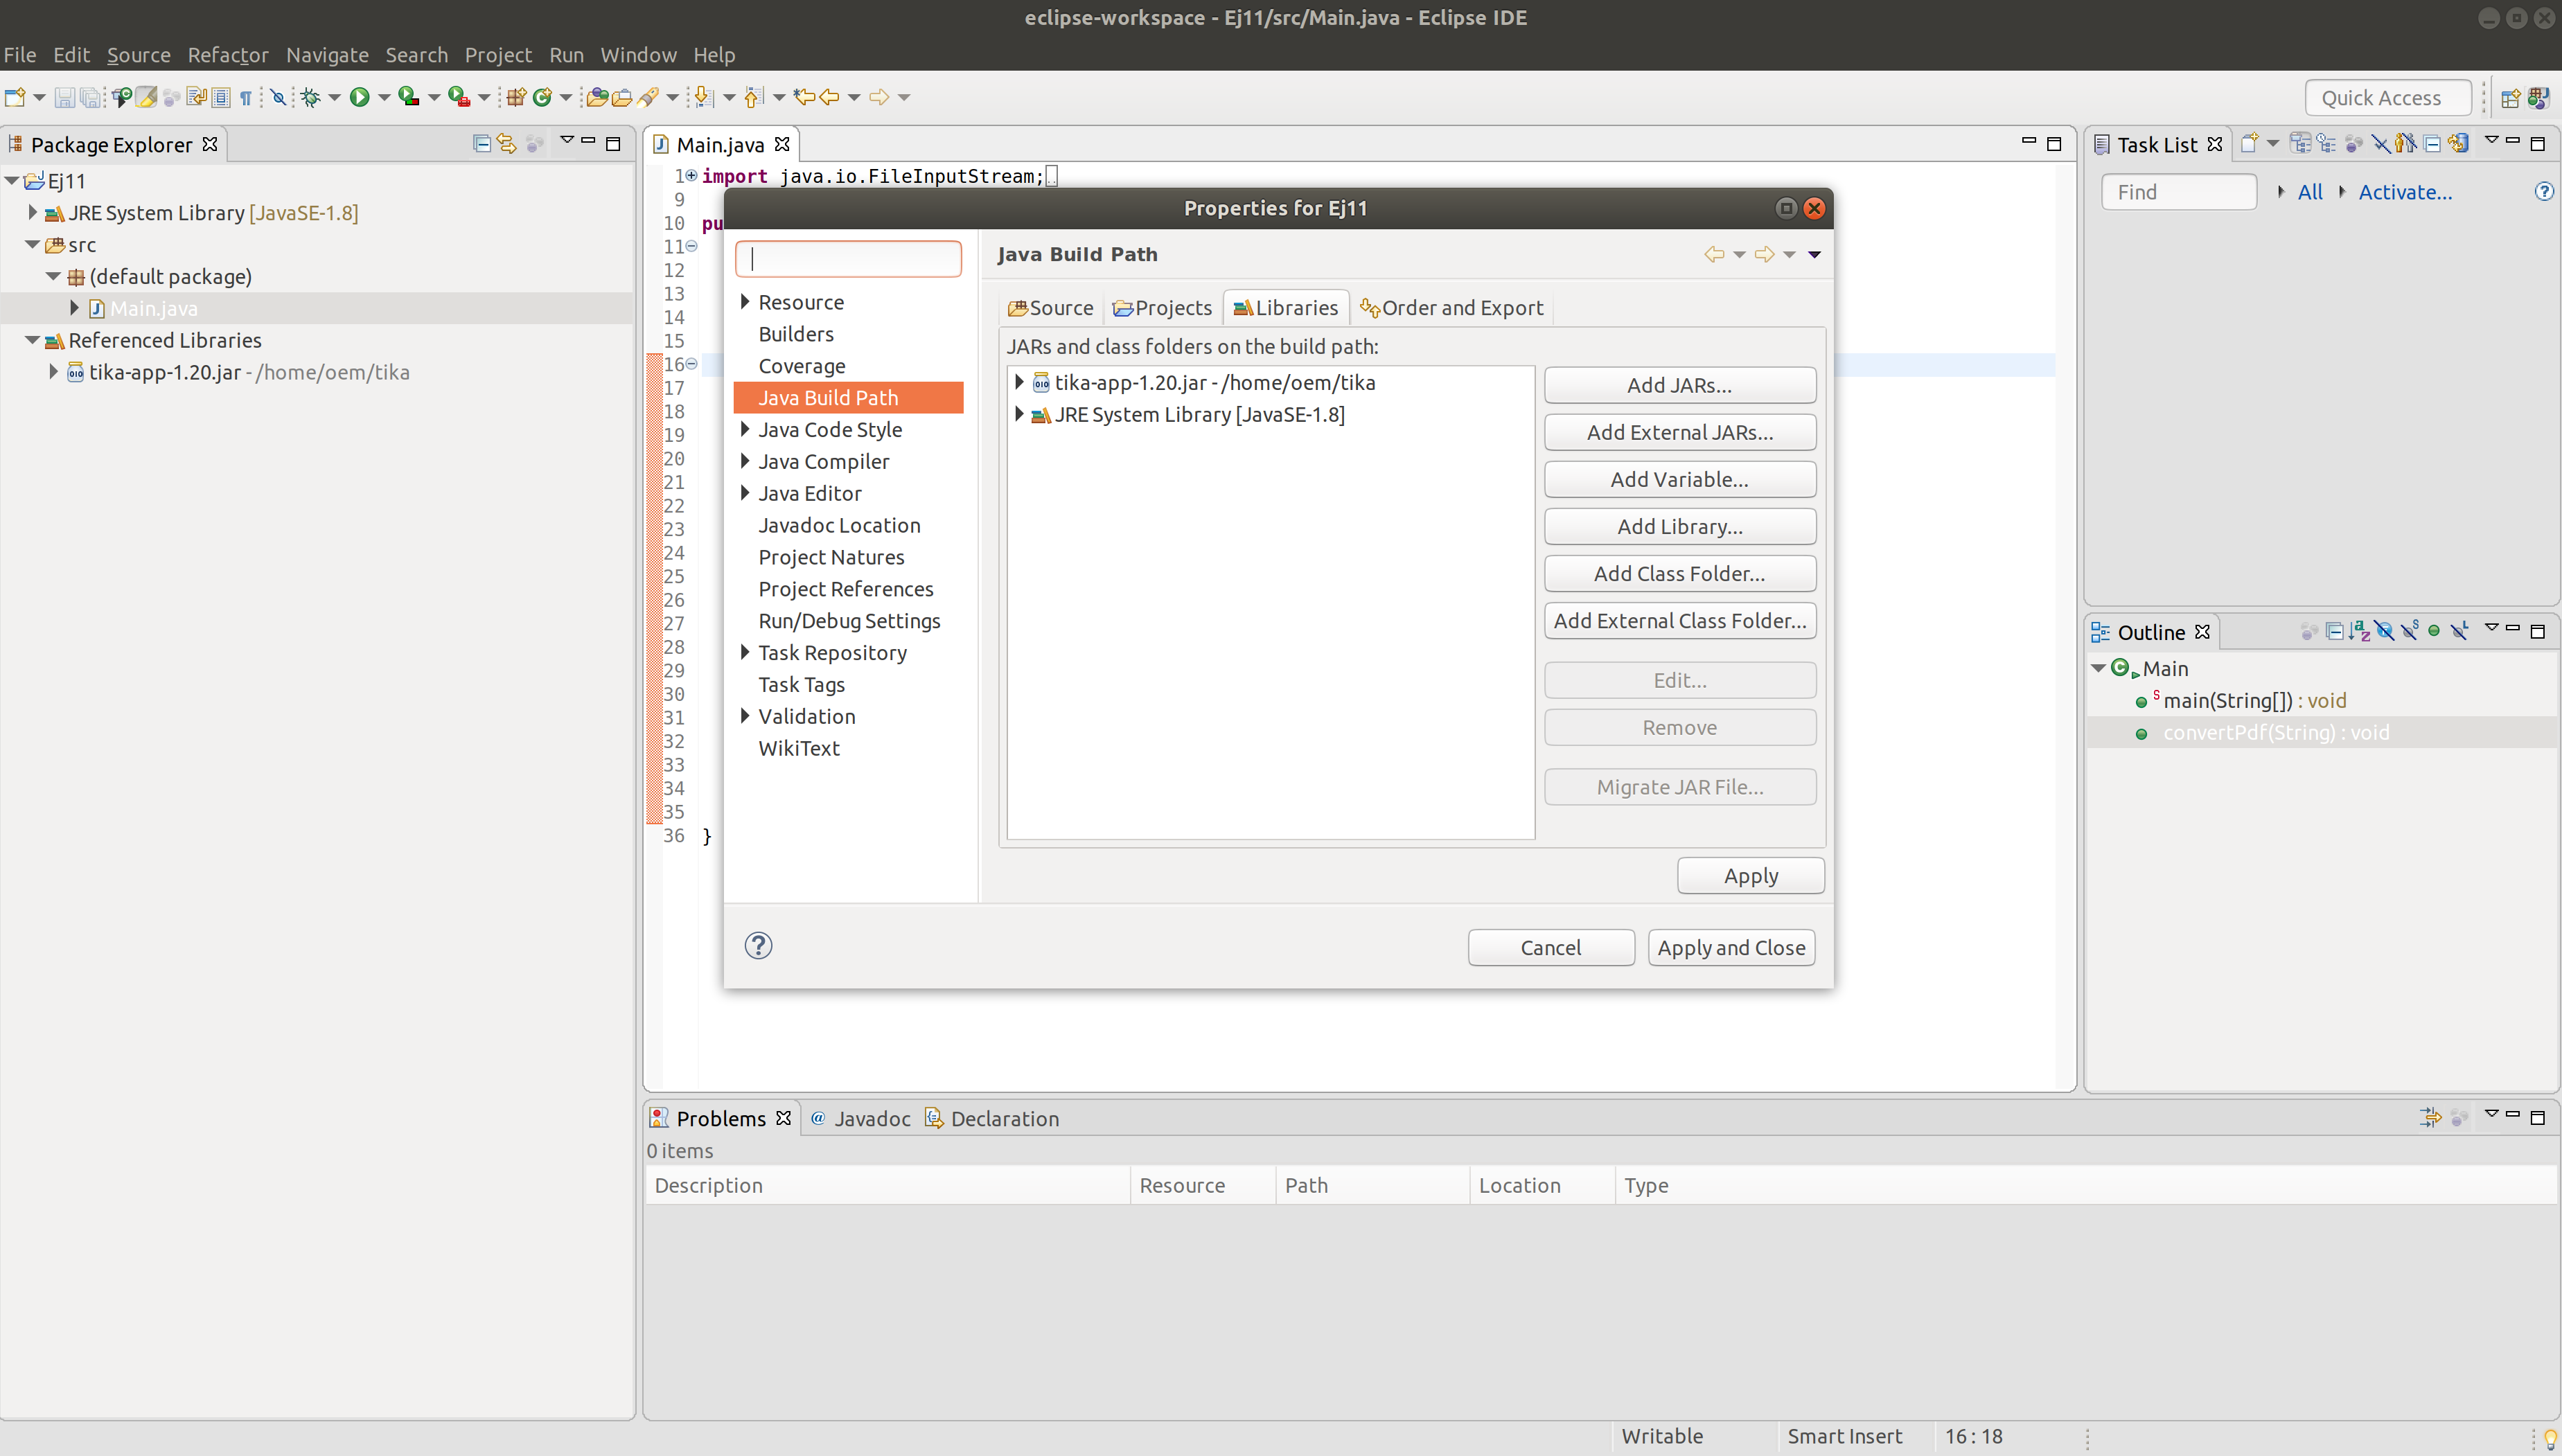
\includegraphics[width=0.7\linewidth]{./ej18}
                \caption{Ejercicio 11.}
                \end{figure}
            \item Seleccionar el jar de la app de tika descargado de la web.
            \item Crear un archivo Main.java donde crearemos el código relevante.
                \begin{figure}[H]
                \centering
                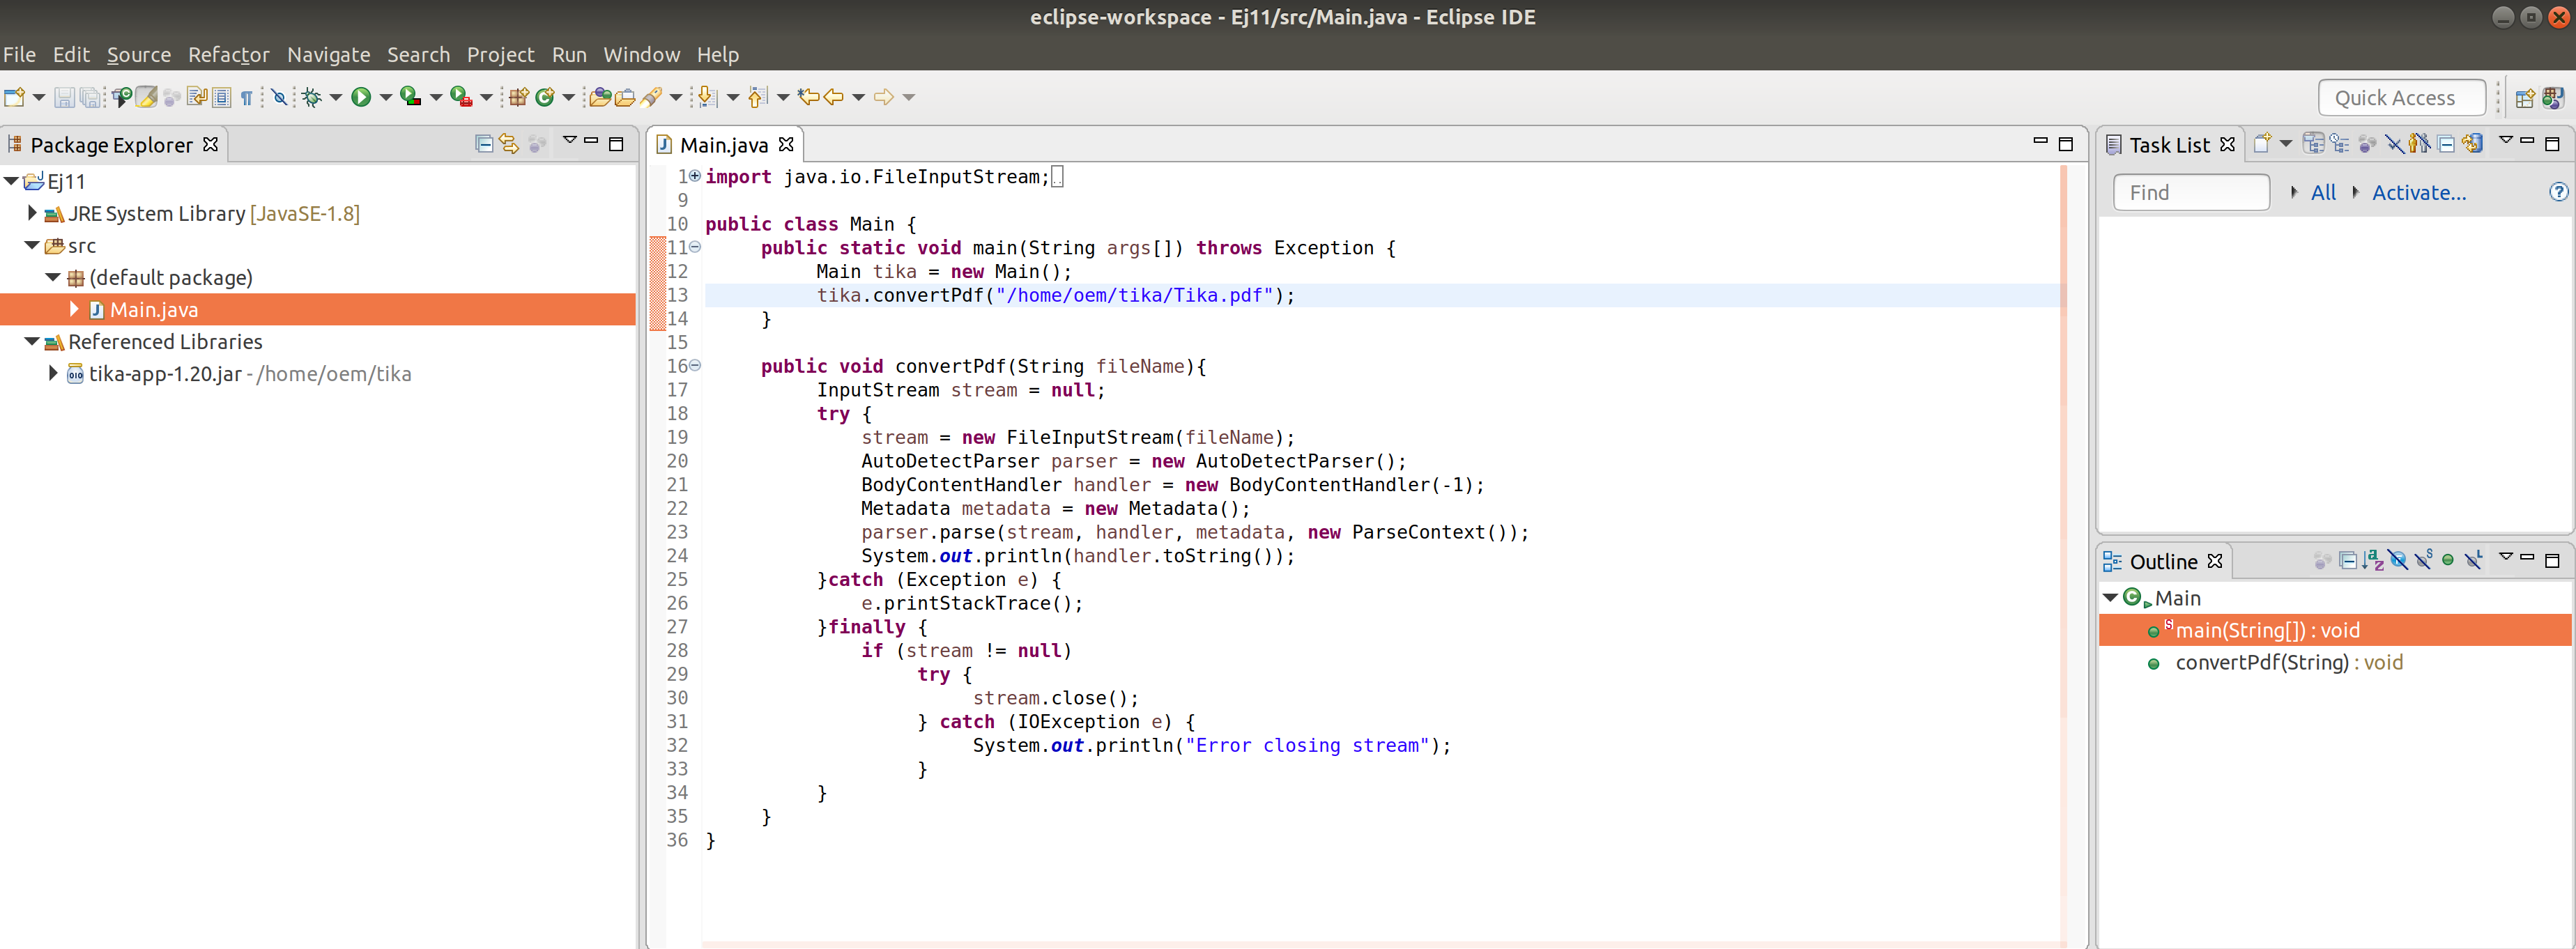
\includegraphics[width=0.7\linewidth]{./ej19}
                \caption{Ejercicio 11.}
                \end{figure}
            \item Guarda el código relevante.
            \item Ejecutar el código relevante.
                \begin{figure}[H]
                \centering
                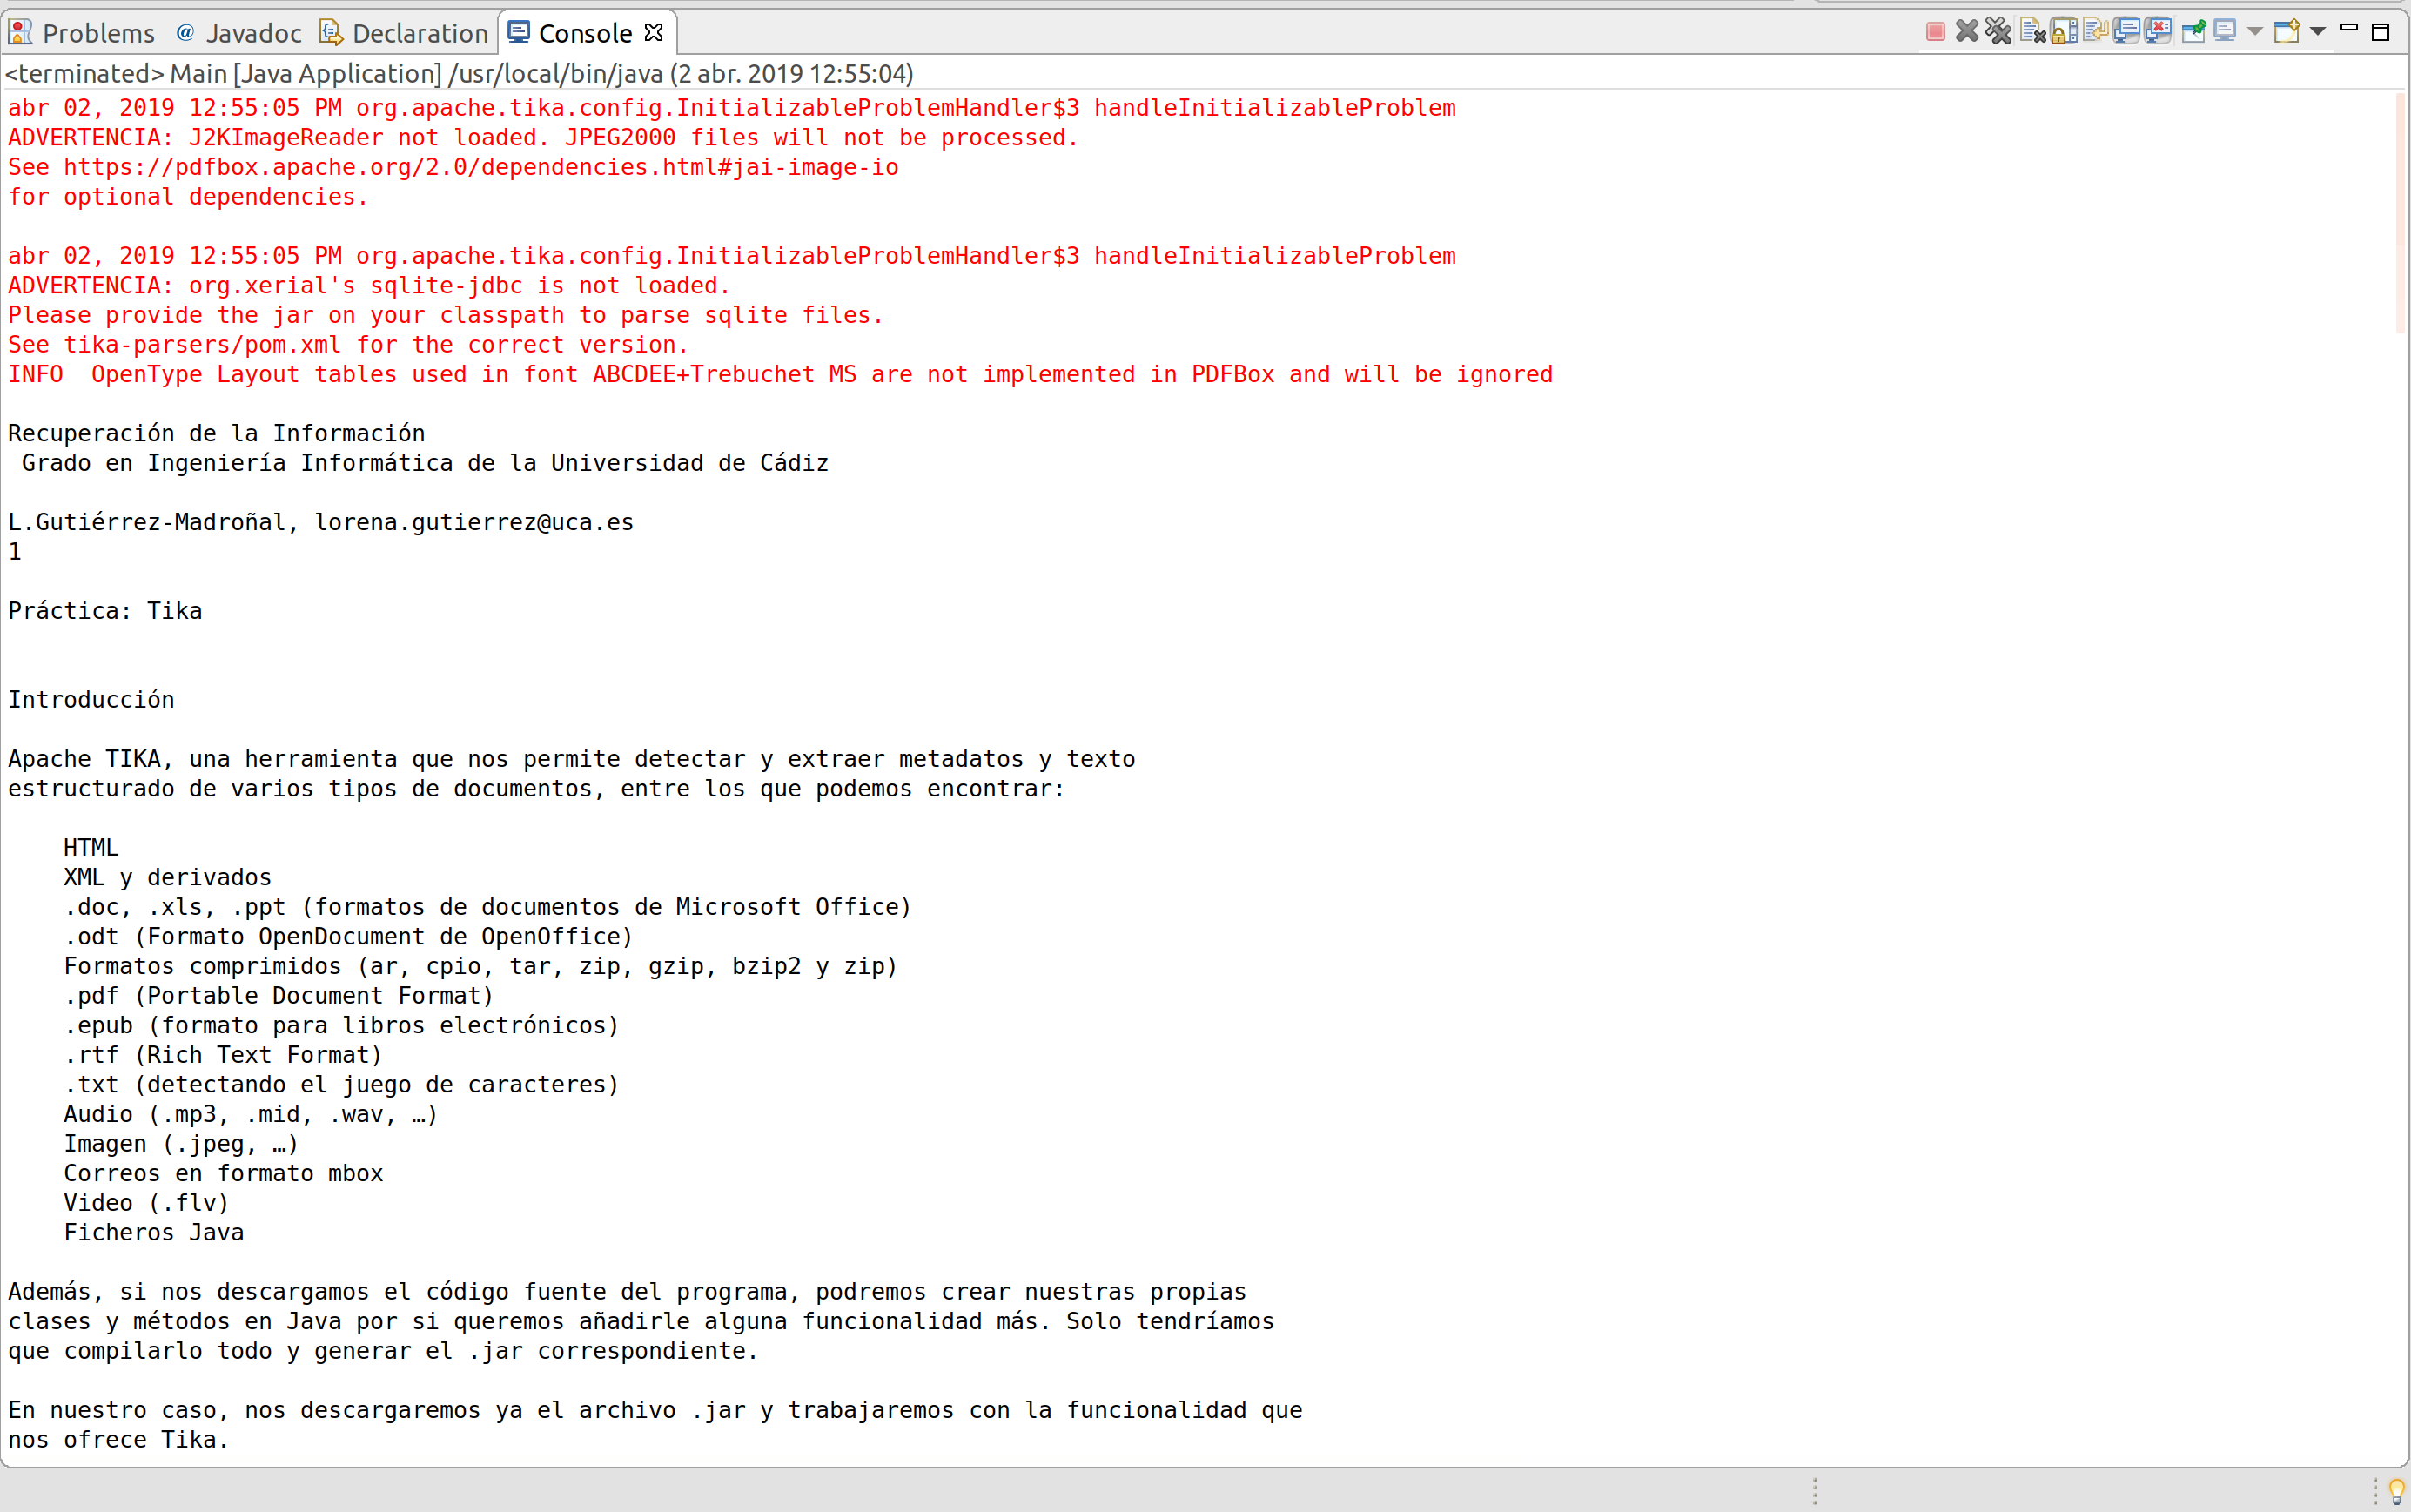
\includegraphics[width=0.7\linewidth]{./ej20}
                \caption{Ejercicio 11.}
                \end{figure}
        \end{enumerate}
\end{enumerate}

\end{document}
